\documentclass[dvipsnames]{interact}



\usepackage[utf8]{inputenc} \usepackage[english]{babel}
\usepackage{csquotes}


% Use times to avoid font missing warnings 
\usepackage[T1]{fontenc}
\usepackage{newtxtext,newtxmath} 






\usepackage{etoolbox} 

\newrobustcmd{\wptitle}{Release management in contemporary digital ecosystems. - Lessons from the OpenStack community}




\newrobustcmd{\wpasin}{As submitted to the special issue on Orchestration in Contemporary Software Development form the European Journal of Information Systems, Aug. 2018.}



\newrobustcmd{\wprunningauthors}{}
%\pdfstringdef{\wprunningauthorsPDF}{}




\newrobustcmd{\wppaurl}{\url{http://www.jteixeira.eu/pub/wp/ICSOB2017SEESNA.pdf}}
  

\newtoggle{bibtex_natbib}
\settoggle{bibtex_natbib}{false}


\newtoggle{biber_biblatex}
\settoggle{biber_biblatex}{true}




\newtoggle{IS-research}
\settoggle{IS-research}{true}

\newtoggle{SE-research}
\settoggle{SE-research}{false}






\iftoggle{bibtex_natbib}{
  \typeout{On bibtex_natbib mode for bibliographies}
}{} 


\iftoggle{biber_biblatex}{
  \typeout{On biber_biblatex mode for bibliographies}
}{} 


\iftoggle{bibtex_natbib}{
  \iftoggle{biber_biblatex}{
    \typeout{ERROR: Chose among packages and pre-processors of bibliographies}
    \typeout{Either bibtex_natbib or biber_biblatex}
    \stop}{} 
}{} 



\iftoggle{bibtex_natbib}{
}{ \iftoggle{biber_biblatex}{}
  {
    \typeout{ERROR: Chose one package and pre-processor of bibliographies}
    \typeout{Either bibtex_natbib or biber_biblatex}
    \stop
  }
} 












\iftoggle{biber_biblatex}{
    
         \usepackage[style=apa,backend=biber,natbib=true]{biblatex}
   \DeclareLanguageMapping{english}{english-apa}
      \addbibresource{./references.bib}

    \addbibresource{./JoseTeixeiraPub.bib}
    \addbibresource{./release-management.bib}
    \addbibresource{./OpenStackResearch.bib}
     \addbibresource{./floss.bib}
     \addbibresource{./extra.bib}
    }{ \typeout{Use biber_biblatex in APA for EJIS} \stop} 

  
\theoremstyle{plain}\newtheorem{theorem}{Theorem}[section]
\newtheorem{lemma}[theorem]{Lemma}
\newtheorem{corollary}[theorem]{Corollary}
\newtheorem{proposition}[theorem]{Proposition}

\theoremstyle{definition}
\newtheorem{definition}[theorem]{Definition}
\newtheorem{example}[theorem]{Example}

\theoremstyle{remark}
\newtheorem{remark}{Remark}
\newtheorem{notation}{Notation}





\usepackage[tikz]{bclogo}
\usepackage{calc}
\usepackage[nomessages]{fp}
\newcommand{\InsertHere}[4]{
\begin{bclogo}[couleur = blue!30, arrondi = 0.1, logo=\bctrombone, barre = none, marge=5]{{#1} {#3}}
\vspace{#4pt}
{#1} {#3} \textbf{#2} to be inserted here.
\vspace{#4pt}
\end{bclogo}
}




\usepackage{array}

\usepackage{multirow}



\usepackage{microtype} 

% To avoid warnings on floats
    \emergencystretch20pt   % More blank space to put in to lines
    \tolerance1000          % value for degree of inadequate line filling


 




 

\usepackage{multicol}




\usepackage{tabularx}
\usepackage{booktabs}

 \usepackage{enumitem}





\usepackage{numberedblock}


 \renewcommand\blocklabel[1]{}

 
 


\usepackage[printonlyused]{acronym}






\newtoggle{boxSubmittedContent}


\togglefalse{boxSubmittedContent} 
 

 
 

\newtoggle{showLiteratureDigests}


\togglefalse{showLiteratureDigests} 
 
 
 
\newtoggle{finalToSubmit}


\togglefalse{finalToSubmit} 
 
 
 
 
 



\newif\ifTaFigOnEnd


\TaFigOnEndfalse 






\newtoggle{showOrgDescription}


\togglefalse{showOrgDescription} 





\usepackage{xargs}






\newcommandx{\error}[2][1=]{\todo[linecolor=red,backgroundcolor=red!50,bordercolor=red,#1]{#2}}
\newcommandx{\unsure}[2][1=]{\todo[linecolor=red,backgroundcolor=red!25,bordercolor=red,#1]{#2}}
\newcommandx{\change}[2][1=]{\todo[linecolor=blue,backgroundcolor=blue!25,bordercolor=blue,#1]{#2}}
\newcommandx{\info}[2][1=]{\todo[linecolor=green,backgroundcolor=green!25,bordercolor=green,#1]{#2}}
\newcommandx{\improvement}[2][1=]{\todo[linecolor=green,backgroundcolor=green!25,bordercolor=green,#1]{#2}}
\newcommandx{\thiswillnotshow}[2][1=]{\todo[disable,#1]{#2}}






\newenvironment{drafte} {\color{violet}}


   
\newcommand{\draftp}[1]{\textcolor{violet}{#1}}  




\usepackage{stackengine}
\setstackgap{L}{.5\baselineskip}
\newcommand\markabove[2]{{\sffamily\color{red}\hsmash{$\uparrow$}  \smash{\toplap{#1}{\scriptsize\bfseries#2}}}}
\newcommand\markbelow[2]{{\sffamily\color{red}\hsmash{$\downarrow$}  \smash{\bottomlap{#1}{\scriptsize\bfseries#2}}}}
  





\newcommand{\boxreview}[2]{\parbox{\linewidth}{
\vspace{0.2cm}
\scriptsize\bfseries\sffamily\color{red}{#1} commented -- {#2}}
\vspace{0.2cm}
}  






   
\newcommand{\newPara}[1]{\textcolor{Sepia}{#1}}  



\newenvironment{newStuff}{
    \begin{color}{Sepia}
    \begin{tabular}{|p{1.0\textwidth}|}
    \hline\\
    }
    { 
    \\\\\hline
    \end{tabular} 
    \end{color}
    }





\usepackage[many]{tcolorbox}
\usepackage{marginnote}
\usepackage{framed}
\usepackage{float}







\newtcolorbox[]{subAndRevbox}[3][]
{
  colframe = #2,
  colback  = #2!10,
  coltitle = #2!20!black,  
  fonttitle=\bfseries\color{Brown},
  title    = \footnotesize  #3,
  #1,
}



\iftoggle{boxSubmittedContent}{    
    \newtcolorbox{submittedText}[1][]{
  oversize,
            breakable,
  enhanced,
  before upper={\parindent15pt},
  colframe=Melon,
  colback=Melon!10
  #1}
  }
  {   \newenvironment{submittedText}{}{}
  }
 
\newtcolorbox[]{submittedNote}[1][]
  {title= \footnotesize {Under review},
   width=3cm,
   left=0pt,
   right=0pt,
   fonttitle=\bfseries\color{Brown},
   colframe=Melon,
   colback=Melon!10,
   #1
}    


\newcommand\submittedTextNote[1]{

  \iftoggle{boxSubmittedContent}{    
    \marginnote[]{    \makebox[0pt][l]{\begin{submittedNote}
    \footnotesize \centering Submitted to #1 
    \end{submittedNote}}}  
 
  }
  
  {    }

}







\newenvironment{submittedFigure}[1][Submitted somewhere]
    {        \iftoggle{boxSubmittedContent}{      \centering 
            \begin{minipage}{1.0\textwidth}
            \begin{subAndRevbox}{Melon}{ \centering Figure as submitted to #1}
      }
      {      }

  }
  {    
       \iftoggle{boxSubmittedContent}{            
      \end{subAndRevbox}             \end{minipage}
       
      }
      {      }
}




\newenvironment{submittedTable}[1][Submitted somewhere]
    {        \iftoggle{boxSubmittedContent}{      \centering 
            \begin{minipage}{1.0\textwidth}
            \begin{subAndRevbox}{Melon}{ \centering Table as submitted to #1}
      }
      {      }

  }
  {    
       \iftoggle{boxSubmittedContent}{            
      \end{subAndRevbox}             \end{minipage}
       
      }
      {      }
}





\usepackage{fixfoot}

\usepackage{tcolorbox}



\newrobustcmd{\PaperTip[1]}{
    
    \begin{tcolorbox}
    \footnotesize \centering {\color{blue}TIP:} #1 
    \end{tcolorbox}
}

\newrobustcmd{\IntroductionCriticalReviewTips}{


\begin{tcolorbox}
\DLquote{''The  purpose of
 this  paper is to stimulate  reflection on the implications of
 the research approaches we as researchers employ when  \textbf{we investigate  information
systems phenomena}``} \citep{Orlikowski_and_Baroudi1991}. --- Nice way to introduce a critical review paper.
\end{tcolorbox}



\DLquote{''The  paper  is structured  as  follows.  In  the first  section  we detail  the  results  of  a
survey which provides evidence for a collective research tradition within the informa-
tion systems
 field,
 and discuss why
 we
 believe such a single philosophy toward study-
ing information  systems phenomena can be limiting. In the following two sections
 we
describe and illustrate two other philosophical research traditions which we consider
to be  valuable  approaches to  studying  information  systems and  their  development
and  use in organizations. We conclude with some general recommendations  for the
information  systems community.``} \citep{Orlikowski_and_Baroudi1991}. --- Nice last paragraph for the introduction of a critical review paper.

}

  
\newrobustcmd{\ResultsTips}{
\begin{tcolorbox}
Jose Teixeira tips for a winning results section:

\textbullet 
The results section should not engage with the literature at all -- that should be relegated to the discussion section. However, when presenting results, take in mind who are the potential reviewers, and add some hooks (i.e. briefly mention literature). It up to you to add small/micro discussions with literature potentially published by potential reviewers. Limit such micro discussion to papers from the target journal, the editors that are the most probable reviewers. 

The use of footnotes or endnotes, and the use of the cf. abbreviation in citations can be useful to introduce such micro discussions. 

Do not forget to mention such scholars in the cover letter. Also do not forget to discuss such hooked micro-discussions in the discussion section. 
\end{tcolorbox}
}  
  
\newrobustcmd{\DiscussionTipsEmpiricalPaper}{

\begin{tcolorbox}
\textbf{Jose Teixeira tips for a winning discussion section:
}


\textbullet  Consider the following \textbf{subsections} for the discussion of a empirical paper: 

\begin{itemize}
 \item What we did, what we learned, and what is the value added of this research (perhaps before opening the subsections)
 \item  \textbf{Key results/findings} and integration with prior literature
 \subitem Integration with prior literature starts with what was confirmed 
  \subitem Integration with prior literature continue with what we extend 
   \subitem Integration with prior literature starts with what we see or propose as new 
\textbf{ \item Theoretical contributions
 \item Methodological contributions 
 \item Practical contributions 
 \item Limitations 
 \item Future research }

 
 
\end{itemize}

\textbullet Leave societal impact issues to the conclusion 


\textbullet  If you have some hooked micro-discussions in the results section.  Do not forget to expand them in the discussion section. If they are relevant to non-experts on the area, mention them in the conclusion as well. 

\textbullet Always look back to the literature that was reviewed, after-all you should be standing on that is already in the literature. 

\textbullet You can use color schemes to better link the associated parts across the Literature, Results and Discussion sections.  
\end{tcolorbox}
}  
  
\newrobustcmd{\ConclusionTips}{
\textbullet 
\begin{tcolorbox}

Jose Teixeira tips for a winning conclusion section:

\end{tcolorbox}

}
  

  




\iftoggle{finalToSubmit}{
\renewenvironment{newStuff}{}{}
\renewcommand{\newPara}[1]{#1}  
\renewcommand{\boxreview}[2]{}
\usepackage[disable,prependcaption,textsize=tiny]{todonotes}


}{


\usepackage[colorinlistoftodos,prependcaption,textsize=tiny]{todonotes}

}





\usepackage{epigraph}

%\usepackage{hyperref} 

\usepackage{cleveref} 


\usepackage{footmisc}
\usepackage{fixfoot}

%\DeclareFixedFootnote{\fixFootrepOne}{See \url{https://docs.openstack.org/project-team-guide/introduction.html} for a brief overview of the history of OpenStack as provided by its community.}



\begin{document}



\articletype{Empirical Research}
\title{\wptitle$^\ast$}
\thanks{$^\ast$\wpasin}

\author{
\name{First Author\textsuperscript{a}\thanks{} and  Second Author\textsuperscript{b}}
\affil{\textsuperscript{a} Affiliation 1 \textsuperscript{b} Affiliation 2}
}

\maketitle





% The abstract is now too close to that in the previous paper. Please revise

\begin{abstract} The dictum of ``Release early, release often.'' by Eric Raymond as the Linux modus operandi highlights the importance of release management in open source software development.  
However, there are very few empirical studies addressing release management in this context. 
It is already known that most open source software communities adopt either a feature-based or time-based release strategy. 
Both have their own advantages and disadvantages that are also context-specific. Recent research reports that many prominent open source software projects have overcome a number of recurrent problems by moving from feature-based to time-based release strategies.
In this longitudinal case study, we address the release management practices of OpenStack, a large scale open source project developing cloud computing technologies. We discuss how the release management practices of OpenStack have evolved in terms of chosen strategy and timeframes, and with close attention to processes and tools. We discuss the number of practical and managerial issues related to release management within the context of large and complex software ecosystems. Our findings also reveal that multiple release management cycles can co-exist in large and complex software ecosystems such as OpenStack. 
\end{abstract}



\begin{keywords}
Open-Source Software; Business Ecosystem, Software Ecosystem, Release Management, R\&D Management
\end{keywords}






\section{Introduction}



%\epigraph{There is little support for software release decision}{\textit{Lai Xu \& Sjaak Brinkkemper}} \nocite{XuBrinkkemper2007} .
%\epigraph{Release early, release often}{ \textit{Eric Raymond}} \nocite{Raymond1999,Raymond2001}
%\epigraph{Google Chrome’s rapid release model (Shankland 2011, 2010), which was eroding Firefox’s user base} \nocite{}


% I changed this to start differently from the previous paper. Feel free to reject my suggestion


% Grammarlly checked 28 Aug 
The dictum of ``Release early, release often'' by Eric Raymond as the Linux modus operandi \citep{Raymond1999,Raymond2001}
highlights the importance of release management in open source software development  \citep[see][]{Aberdour2007,SharmaSugumaran_et_al2002,MichlmayrFitzgerald_et_al2015}).  
Across disciplines, release management is acknowledged to be a very complex process that raises many issues among the producers and users of digital technologies 
\citep{XuBrinkkemper2007,AdamsBellomo_et_al2015,BarqawiSyed_et_al2016,ChoudharyZhang2015}.  However, there are very few empirical studies addressing 
release management in open source software development \citep{MichlmayrFitzgerald_et_al2015,PooCaamano2016,Teixeira2017}. 
This is unfortunate since many lessons can be learned from open source software communities \citep{OReilly1999,SpinellisSzyperski2004,Fitzgerald2011} because they allow studying the socio-technical aspects of digital technologies development freely whilst the proprietary model intrinsically restrict the access of scholars.  


% Grammarlly checked 28 Aug 
Given this scarcity of empirical work on release management in the context of open source software \citep{MichlmayrFitzgerald_et_al2015,PooCaamanoKnauss_et_al2017,Teixeira2017},
we address how a particularly large, complex and highly networked open-source digital ecosystem organizes its release management practices. Taking the case of OpenStack, a fast-growing cloud computing platform that is increasingly attracting scholarly attention    \citep[e.g.,][]{CorradiFanelli_et_al2014,CarilloBernard2015,teixeira_et_al_icis2016,armisen2016formative,MalikAhmed_et_al2017}, we detail the release management practices by looking at the overall release management process \textit{per se} as well as the organizational design that supports it. All efforts towards an encompassing theory explaining release management in contemporary digital ecosystems.  

 % Grammarlly checked 28 Aug 
By following the OpenStack digital ecosystem since its inception at the\ac{NASA}, and while getting acknowledged with multiple problems and challenges that confronted the release management team over time, we advance details on the release management process \textit{per see} as well on the organizational design after the digital ecosystem attained some maturity. He found that a cross-project release management team that mixes people from the different feature-development sub-projects jointly with permanent release management staff relies upon freezes to encourage developers to change their production focus from the development of component to the overall upstream integration and stabilization of components as a whole. The release management process incites developers to catch the planned release dates before the project switches from the production to the integration and stabilization mode. We also found that the release management team is tightly integrated with the continuous integration, testing, and peer-review teams, but its the release management team that handles 'what is' an 'what is not' an official OpenStack released. 

% Grammarlly checked 28 Aug 
After many procedural and organizational refinements, OpenStack runs now a time-based release management cycle that is quite permissive, that is, it is open to changes and flexible to adaptation. In particular situations, the different sub-project teams across the community are allowed to work around the 'default' six months release cycle. As the project grew, different release cycles started to co-exist across the various OpenStack sub-projects. Furthermore, as the project grew and the boundaries of the digital ecosystem turned blurry, only projects that are release managed can be considered an official OpenStack release (i.e., can use OpenStack logo and trademark). Lessons from the OpenStack open-source ecosystem highlight the importance of release management and call for further research that could explain how release management should be organized on contemporary digital ecosystems. We remain far from explaining when and how significant changes on digital technologies should be optimally released.  


\section{Theoretical background}

\todo{Should be organized as ``On release and release management'', ``On open-Source digital ecosystems'', ``Release management in open-source software ecosystems ''}


\subsection{On release and release management}




\begin{color}{Blue}

The most central concept to this research is the one of \textit{release}. It is a concept that is often misunderstood in the development of digital technologies \citep{HoekHall_et_al1997,LahtelaJantti2011,Howard2016}. After all, in this kind of context, a \textit{release} can be seen as a raw chain of binary digits that move around, but not necessarily being visible to its users.

In our view, there is established literature targeting practitioners that merit both by introducing the \textit{release} concept and highlighting the importance of the \textit{release management} process. 
For example, the ITIL framework\footnote{The ITIL (Information Technology Infrastructure Library) framework, originally  developed by the Central Computing and Telecommunications Agency (CCTA) of the UK government, details a catalog of practices for digital services management that focuses on aligning digital services with the needs of business. See \citep{McNaughtonRay_et_al2010,GorlaSomers_et_al2010} for Information Systems research related to ITIL.}  defined \textit{release} as a 'set of authorized changes' \citep{GovernmentCommerce2005},  'a significant change' \citep{Bon2011} and 'one or more changes that are built, tested and deployed' \citep{Davies2016} in the context of digital services. 
Furthermore, and pertaining the specific context of software development, the following quote 
from the \textit{ Software Engineering Body of Knowledge (SWEBOK Guide)}
% I do not think this footnote is needed
%\footnote{The (SWEBOK Guide), published and made publicly available by the IEEE Computer Society, describes generally accepted knowledge about software engineering.}  
provides valuable insights on what \textit{release} means: 


\begin{quotation}
 ''release refers  to  the  distribution  of  a  software  configuration  item outside the development activity. 
This  includes  internal  releases as well as distribution to customers. When  different versions of a software item are available  for  delivery  (such  as  versions  for  different  platforms  or  versions  with  varying  capabilities),  it is  frequently necessary to recreate specific versions  and  package  the  correct  materials  for  delivery  of   the version.``  ---  \citep{Society2014}
\end{quotation}
% the citation should be to Bourque & Fairley 2014


When introduced to practitioners that develop and deploy digital technologies, the concept approximates the \textit{Oxford English Dictionary} definitions of \textit{release} [VERB]  as 
``Allow or enable to escape from confinement; set free.'',
``Allow (information) to be generally available.'',
``Allow (something) to move, act, or flow freely.'',
``Remove restrictions or obligations from (someone or something) so that they become available for other activity.'';
and \textit{release}  [NOUN] as  ``The action of making a film, recording, or other product available to the public.'' and
``The action of releasing property, money, or a right to another.''. 


Across computing disciplines, scholars have provided definitions of  \textit{release} as 'a new version of an evolving product' \citep{Ruhe2005}, 'passing artifacts on to one or more parties outside of the development' \citep{Ould1999}, 'a decision to distribute code for testing or operation' \citep{PortWilf2013},   'deployment of a version of a product' \citep{DidarAlAlamKarim_et_al2016} or 
``to package and make a software system available to a customer'' \citep{HoekHall_et_al1997}. It is worth noting that existing views on 'what is a release' are somewhat contradictory. Some definitions emphasize the flow of artifacts to customers or users, while others emphasize distinct 'crafting' practices that each release encompasses.


\end{color}




\begin{newStuff}
 Two paragraphs on what is release management are Not ready 



 Release management is then concerned with the overall management of all tasks concerning planning, building, testing, version control and configuration management (van de Weerd et al. , 2006)
 IN EJIS

 Release management is not release planning, release engineering or release maintenance, 
 
 One concept that clarifies the difference between release management and project management is that there can be many projects in one release. \citep{Howard2016}.

  
  
\end{newStuff}


\begin{newStuff}
 
 Release increments . they accumulate less bugs due to the shorter release cycle\citep{KhomhAdams_et_al2015}, being less effective at triaging bugs with rapid release, I’m not surprised that fewer bugs are fixed: some defects are trivial and some will take weeks of careful code inspection to find and fix. All those bugs would have fallen in the same bucket for a 12+ month release cycle, but now the harder ones get pushed out to later releases
 t “some users don’t like the frequent changes and want their product to be more ”stable””\citep{KhomhAdams_et_al2015} 
 
 
 
 Release big changes. leads to accumulated more bugs, \citep{KhomhAdams_et_al2015} 
 
 
 
\end{newStuff}



\iftoggle{SE-research}{
Across computing disciplines, but predominantly in software engineering, plenty of research has addressed issues of release management (see \citep{MullerHerbst_et_al2006,StarkOman_et_al1999,Ruhe2005,Jrgensen2001,Wright_et_al2012,ClevelandEllis2014,LaukkanenPaasivaara_et_al2018} among others).
}{}

\iftoggle{IS-research}{
Across disciplines plenty of research has addressed issues of release management (see \citep{MullerHerbst_et_al2006,StarkOman_et_al1999,Ruhe2005,XuBrinkkemper2007,IravaniDasu_et_al2012,ClevelandEllis2014,ChoudharyZhang2015,LaukkanenPaasivaara_et_al2018} among others).
}{}



Whilst we acknowledge and value such research, we note that the studies were mostly conducted in single firms that released proprietary software; a sharp contrast with our case where multiple firms release open source software.  

There is a recent framework for analyzing openness in the context of digital platforms and ecosystems \citep{Teixeira2015}, which raises issues of governance, transparency, market and intellectual property that can be used to juxtapose release management on the single firm releasing proprietary software vs. the network of firms releasing open source software. We revisit the framework here:  

\begin{itemize}
 \item \textit{Governance}.  There is a sharp contrast in terms of inclusiveness and control across these two settings. While a single firm releasing proprietary software has more control over its development processes, the network of firms needs to accommodate multiple and often conflicting agendas. Release management in open source software ecosystems needs to accommodate that participants can have different and competing business models and thereby different motivations to engage and contribute. Furthermore, release management in open source projects is more exposed to different mental models, different corporate and individual cultures in a setting, or 'irrevocable openness' \citep{Howison_and_Crowston2014}. 
 In addition, open source ecosystems also tend to be more inclusive to third-party contributors (e.g., students, academics or users among others that do not need a certain organizational affiliation or license to contribute). The power and the influence on deciding what is and what is not released are shared across multiple and heterogeneous participants \citep{Teixeira_et_al2015}. 
 
 \item \textit{Transparency}.  While it is common for the single firm releasing proprietary software to hide information about the software being released (e.g., the source code, the bug tracking information), the same is not customary in open source software ecosystems, where access and transparency are required for the community to function. It is also worth remarking that while most open source software is released on the Internet (i.e. to a repository or a website where it can be consumed by others), much proprietary software is only considered released when deployed in the customers' production environment \citep{LaukkanenPaasivaara_et_al2018}.
 
 \item \textit{Market}. While a single firm releasing proprietary software has more control over the commercialization of the software and its complements, in the case of open source software ecosystems, the value exploration around a component is out of the control of a single firm. Multiple firms can compete for the value around the 'common' software being released. In the case of OpenStack, when deciding whether a certain open source component is released or not, a number of issues can be raised, such as 'Will the component compete with some of our proprietary offerings (e.g., plug-ins)?', 'Will the component allow us to win some consulting and deployment contracts?', 'Will the component increase the demand for our hardware?'or 'Will the component increase the demand for our hosting infrastructure?'  among other market-related issues that can impact release management.

 \item \textit{Intellectual property rights}. Releasing software can create \textit{prior art} in terms of intellectual property rights. Single firms releasing proprietary software tend to deal more with intellectual property protection issues. In open software ecosystems, there might be intellectual property issues as well, but they often need to be resolved across multiple participants. Furthermore, by releasing under an open source software license, the developers or firms are giving up rights that are automatically granted by law. Note that it is not uncommon for firms to submit related patents prior to releasing a certain software component. This aspect is more relevant in markets where software can be patentable (USA, Japan, and South Korea) \citep{HallMacGarvie2010}. From the point of view of brands and trademarks, there is also a sharp contrast. While a single firm often has control over the trademark of a given software product, in the case of open source software this kind of control is often multilateral and negotiated across the different individuals and organizations that contribute to the joint development of open source software. After all, the quality of a given release can affect the value of the brand and the trademark associated with the software being released.  


\end{itemize}


\subsection{Release management in open source software ecosystems}
 

Within the specific context of open source software, release management affects both producers and users of software. On the producer side, prior research has shown how community activity increases when the scheduled release date gets closer \citep{RossiRusso_et_al2009}. On the user side, new releases can result in spikes of downloads \citep{WigginsHowison_et_al2009}. \begin{newStuff}Library projects where new code libraries are developed and client projects where the libraries are reused, organize release management in a different way to accomodate their technical dependencies.\end{newStuff} Recent results  suggest that client projects are quicker to update libraries with a rapid release cycle compared to actual library projects with a longer release cycle \citep{IharaFujibayashi_et_al2017}.  The same study also suggests that client projects are more likely to adopt the latest version of libraries with shorter release cycles.
As noted in the early work of Michlmayr on open source software \citep{Michlmayr2007}, release management is concerned with the delivery of products to end users. It is therefore not surprising that recently some have seen release management as a process that supports value co-creation among suppliers and consumers of software \citep{ClevelandEllis2014,BarqawiSyed_et_al2016}. 

As pointed out by three recent doctoral dissertations addressing release management in the context of open source software  \citep{Michlmayr2007,Wright2012,PooCaamano2016}, 
most open source software communities adopt either a feature-based or a time-based release strategy. Many prominent open source software projects start with sporadic releases in which developers announce the newly developed features\footnote{See the historical newsgroup \url{news:comp.os.linux.announce} where developers announced new releases of open source software for Linux with a strong emphasis on the implemented features.}. However, as many of these projects grew in size and complexity, they started adopting time-based release strategies\footnote{See  \url{https://www.kernel.org/category/releases.html}  and 
\url{https://www.debian.org/releases/} for information on the releases of Linux (2-3 months release cycle) and Debian (with a two years release cycle).}. 
An early empirical study \citep{MartinezRomoRobles_et_al2008} that mined the repository of a project while it adopted a time-based release strategy (i.e., the evolution of an e-mail client),  reported that the adoption of a time-based release cycle boosted the development in general terms over time in comparison to feature-based release cycles. 
There are many problems associated with feature-based strategies. For example, if critical features are not ready, they block the overall release.  Another example is when developers work on the features they are interested in, coordinating their activities can be challenging \citep{Michlmayr2007}.
Recent studies based on interviews with key members of seven prominent volunteer-based open source projects, point out that these problems can be overcome by employing a time-based release strategy \citep{MichlmayrFitzgerald2012,MichlmayrFitzgerald_et_al2015}. 

Time-based release strategies encompass meeting a schedule, an agenda, or a deadline. These can be either strict or liberal.  To enforce that software is released on time, the use of freezes (such as code freezes) will set a clear deadline for the software development team.  Open source developers have much freedom to manage their own software development efforts, but the use of freezes acts in the opposite way, by constraining the developers. If new features are not implemented before the upcoming freeze, they will not be included in the next release. Consequently, when developers realize this, the development of these features is either canceled, put on hold, or developed separately for future releases.

The freezes that occur before the scheduled time-based release, act as control mechanisms that slowly halt the production of the development core code \citep{Fitzgerald2011,AnandBhatt_et_al2017}. In large and complex open source software projects with a modular architecture integrating components with each other, this kind of a freeze forces developers to (1) fix and release the individual components upstream, (2) integrate the different components and test the integrated totality.  

According to Fitzgerald, the freeze categories can include \citep{Fitzgerald2011}: 
\begin{description}[leftmargin=!,labelwidth=\widthof{\bfseries feature freeze}]
\footnotesize
 \item[feature freeze] no new functionality can be added, the focus should be on removing defects;
\item[string freeze] no messages displayed by the program, such as error messages,  can be changed. This allows translating as many messages as possible before the release; \footnote{Here we add that many automated user interface testing tools and techniques depend on the stability of certain strings (see \citep{MesbahVanDeursen2009,ArtziDolby_et_al2011}) as well.}
\item[code freeze] a permission  is required to make any changes, even to fix bugs.
\end{description}


\begin{color}{Blue}
While the freeze mechanisms seem to be widely employed across the open source community, the practice of release management largely varies across projects. As pointed out in on a comprehensive review of research on open source software by \citet{Crowston_and_Howison2008}, large open source software ecosystems such as Apache, Subversion, Linux, or FreeBSD largely differ  on how software releases are scheduled, tested, organized, or distributed \citep{Glance2004,Crowston_and_Howison2008,Erenkrantz2003,MichlmayrFitzgerald_et_al2015,Teixeira2017}. To our view, this kind of variance remains largely unexplained and  calls for further theorizing.  To that end, we offer a detailed description of release management at the OpenStack open source software ecosystem by employing both processual and organizational views.  Given the trans-disciplinary nature of Information Systems \citep{Galliers2003,CarilloBernard2015}, the field would be in a good position to engage in a dialog, contributing to a cumulative body of knowledge that integrates ideas and concepts from Software Engineering and Management.  


\end{color}



 





\section{Empirical background}


The cloud computing business is dominated by a small number of players (e.g., Amazon, Google and Microsoft). The leading players do not sell cloud infrastructure products. Instead, they provide bundled computing services. If there was no alternatives, all cloud computation would run in hardware and software infrastructures controlled by very few players with increased customer lock-in \citep{Teixeira_et_al2015}. 

Competing with the providers of these services, the leading product alternatives are not commercial. Instead, they are four open source projects: OpenStack, CloudStack, OpenNebula, and Eucalyptus. While the commercial cloud computing services are developed and tightly controlled by a single organization, the open source products are more inclusive and networked where multiple firms participate in their development and where multiple firms attempt to capture value from them.

OpenStack is an open source software cloud computing infrastructure capable of handling big data. It is primarily deployed as an ``Infrastructure as a Service'' (IaaS) solution.  It started in 2010 
as a joint project of Rackspace, an established IT web hosting company, and NASA, the U.S. governmental agency responsible for the civilian space program, aeronautics and aerospace research.  As it evolved,  the project attracted much attention from the industry. 
By the end of 2017, OpenStack counted with more than 82 000 contributors and 670 supporting companies in 187 countries. \footnote{See \url{http://www.openstack.org/} for the official website.}

Both private companies (e.g.,  AT\&T, AMD, Canonical, Cisco, Ericsson, HP, IBM, Intel, VMware, Citrix, and NEC,  among many others) and research-intensive organizations (e.g., NASA, CERN, Johns Hopkins University, Instituto de Telecomunicações, Universidade Federal de Campina Grande, and Kungliga Tekniska Högskolan, among  others)  work  together with independent, non-affiliated developers in a scenario of pooled  \ac{RanD}. 
They work in the open source way, that is, emphasizing development transparency while giving up intellectual property rights. Paradoxically, even though OpenStack emphasizes collaboration in the joint development of a large open source ecosystem, many participating firms also compete  with each other. Among others, there is competition among providers of public cloud services based on OpenStack (e.g., HP, Canonical, and Rackspace), among providers of specialized hardware complementing OpenStack (e.g., HP, IBM, and Nebula), and among providers of commercial software plug-ins that complement OpenStack (e.g., VMware, Citrix, and Cisco) (see \citep{teixeira_et_al_icis2016,Teixeira_et_al2015} for related research addressing cooperation among competitors within OpenStack). 

% you should give the market size in 2018, now the reader assumes that this is a paper from 2016 that has been rejected and revised
We decided to address OpenStack due to its perceived novelty, its highly inter-networked nature (i.e., an ecosystem involving many firms and individual contributors), its heterogeneity (i.e., an ecosystem involving both startups and high-tech corporate giants), its market size (\$1.7bn, by 2016\footnote{See \url{http://451research.com/report-short?entityId=82593}.}), its complexity (i.e., involving different programming languages, different operating systems, different hardware configurations) and size (20 million lines of code). 

From the early beginnings of OpenStack, the project  adopted a liberal six-month, time-based release cycle with frequent development milestones that raised much discussion among its developers. We found it an interesting case to study release management within the overlap of open source software, software ecosystems, and complex software systems. 

\section{Methodological design}
\label{sec:method}

This empirical case study was guided by the broad research question on ``How did OpenStack implement a time-based release strategy?'' A particular emphasis was given to the release management process \textit{per se} as well as to the infrastructural tools supporting it. Tools are focal as the OpenStack community attempts to automate the release management process as much as possible \footnote{See \url{https://doughellmann.com/blog/2016/03/15/} for a blog post regarding the process automation efforts by the OpenStack release management team.}. 


Our efforts were built on top of publicly available and naturally occurring archival data derived from the OpenStack project.  
These data are not a consequence of our own actions as researchers, but are created and maintained by the OpenStack community in their own pursuits in developing a cloud computing infrastructure. We took into account many methodological notes in case study research that legitimate the use of archival data when studying a case
\iftoggle{SE-research}{~\citep{runeson2008guidelines,EasterbrookSinger_et_al2008,Yin2011,Eisenhardt1989,FlynnSakakibara_et_al1990}.}{}
\iftoggle{IS-research}{~\citep{Eisenhardt1989,DubePare2003,Flyvbjerg2006,GibbertRuigrok_et_al2008,Yin2011}.}{}



We started by 'digesting' many websites officially related to OpenStack (e.g., \url{https://www.openstack.org/}, \url{https://wiki.openstack.org} and \url{http://docs.openstack.org/}), expanding later to other websites. When selecting the initial sources (i.e., departure points), we took into consideration key guidelines on how to conduct qualitative empirical research online ~\citep{Kozinets2002,Kozinets2009}. From the initial sources, we followed several links to collect further information. The links often led to blogs maintained by organizations and individuals that recurrently contribute to OpenStack. Relevant data was meticulously organized in a database for later analysis \citep[pp 94-98]{Yin1994}. 

From our initial screening of qualitative data, we were able to: (1) make sense of the industrial background in which Openstack is embedded, (2) make sense of the complex software development processes that steer the project evolution, (3) survey complex inter-organizational arrangements within the project,  and (4) understand the role of many of the software tools that support its software development processes. After getting familiar with many social-technical issues within OpenStack, we analyzed the collected data with the lenses of extant knowledge in release management and open source software. 

Given the scarcity of theoretical and empirical knowledge addressing release management in open source software \citep{MichlmayrFitzgerald_et_al2015,PooCaamanoKnauss_et_al2017}, we explore and narrate  the evolution of release management in practice. Our rich narrative on how OpenStack implemented a six-month, time-based release cycle with frequent development milestones, can increase our ability to understand and explain release management within the context of complex open source software ecosystems. 

To enhance the validity of our narrative, we asked four OpenStack developers (two of them with release management responsibilities) to  read and comment our \Cref{sc:process,sc:tools} in advance. One of our informants had joined the project in November 2010 with the responsibility of organizing release management at OpenStack and has reported since then to the \ac{TC} of the OpenStack foundation. Another of our informants joined OpenStack in 2014 and currently leads a sub-project and recurrently attends cross-project team meetings dealing with release management. While the first one has a more managerial view on release management at OpenStack, the second one sees release management from the complementary developers' perspective.   
In this way we reduced possible misinterpretations of the collected data. 
% What about the 2 others?


Our description of release management in the particular case of OpenStack is organized around a dual view that aggregates two different aspects of release management. First, a view on release management as a complex and evolving inter-organizational socio-technical process; and second, an infrastructural view oof the tools that support it. 

\section{Results: a processual view}
\label{sc:process}

% move this to the introduction
% Release management can take many distinct forms and many lessons can be learned from how it is done in an open source software community \citep{Fitzgerald2011}. 

Table with problems 

\newPara{
Given that release management at OpenStack evolves dynamically as a moving target, we organize our narrative across three phases of OpenStack. First, we briefly describe its early days as an internal project of NASA. Then, we look at its bootstrap as an open source software project, largely steered by Rackspace (at that time supplying NASA with cloud computing services). After that, we concentrate our attention on describing release management at OpenStack at a more recent and mature phase (i.e., release management of OpenStack as by the end of the year 2017).  We provide a narrative on the evolution of release management at OpenStack while purposively focusing on its more recent and mature phases from which more lessons can be learned. 
}
%the NASA subsection can be shortened considerably
\subsection{Early days at NASA}
The OpenStack project was officially announced on July 21, 2010 at OSCON (a business and technical oriented convention organized by O'Reilly Media that gathers annually many open source contributors across different cities of USA). However, the technology behind OpenStack started much earlier at NASA  (a well-known space and aeronautics research agency) and Rackspace (a popular provider of hosting services).

At that time,  Anso Labs had published the beta code for \textit{Nova}, a cloud computing fabric controller implemented in the C, C++ and Python programming languages.  Anso Labs was later acquired by Rackspace on February 9, 2011 and since then \textit{Nova} remains a core component of OpenStack. Meanwhile, Rackspace also wanted to rewrite the infrastructure code running its offering for cloud servers, and open sourced the existing cloud files. This open sourcing of code, previously held in-house,  led to the creation of \textit{Swift} that is OpenStack's scalable redundant object storage system. As an open source project, \textit{Swift} was able to address the exceptionally demanding storage needs of NASA. The first release of OpenStack had then two main components: \textit{Nova} and \textit{Swift}. This is how OpenStack started (see 
\cite{teixeira_and_Hyrynsalmi2017icsob} for a more detailed narrative on how OpenStack started at the hands of  NASA, Anso Labs, Rackspace, and others).

These initial software components were not developed in the open source arena but in-house. The software was released once new features were ready. This is in a big contrast with OpenStack today, in terms of release strategy and the overall development transparency.  Nowadays, OpenStack releases trail a six-month release schedule and tarballs\footnote{A compressed archiving format that is very popular within the open source community} are available for every single code commit. In the particular case of \textit{Nova} at NASA, its release management was influenced by procedural requirements at NASA: all software developed in and for NASA should follow comprehensively documented procedures such as  Release Management (SWE-085), SW Development-Management Plan (SWE-102),  and Release of NASA Software (NPR 2210) among many others\footnote{See \url{https://nodis3.gsfc.nasa.gov/} for the NASA Online Directives Information Systems (Agency Level Directives) and \url{https://swehb.nasa.gov/} from the Software Working Group for accessing relevant versions of this kind of procedural documentation.}.

\newPara{
Nowadays, NASA has its own documented procedures on how to release open source software. So far, NASA has released more than 60 software projects under the NASA Open Source Agreement (NOSA), a non-permissive license created and approved by the Open Source Initiative (OSI) in 2013.  Note, however, that in the early days of OpenStack at NASA, the release of software to the open source community was uncommon \footnote{See \url{https://open.nasa.gov/blog/open source-development-at-nasa/} for more information on how NASA has improved its engagement with the open source community.}
}

\subsection{Bootstrap as an open source project}

The mission of OpenStack, in the announcement in July 2010, was to "to produce the ubiquitous Open Source Cloud Computing platform that will meet the needs of public and private clouds regardless of size, by being simple to implement and massively scalable.`` The first OpenStack design summit was held in Austin, Texas, USA during July 2010. The announcement highlighted prior work made in NASA. Citrix, a long standing partner of Rackspace on virtualization technologies,  joined the project.  The project kept growing with more and more partners (e.g., Intel, Cisco, Nebula, CloudScale, HP, Mirantis, Canonical, VMware, RedHat, and IBM among others) and the OpenStack foundation was founded as a non-profit corporate entity, established in September 2012, to manage and promote OpenStack and its community. 
(see \cite{Teixeira_et_al2015,teixeira_and_Hyrynsalmi2017icsob} for more details on how OpenStack open source project grew over time). For protecting the brand, OpenStack holds the trademark and hires staff that deal directly with release management from the development side (engineering, design, infrastructure, ecosystem management, etc.) as well as the marketing side (events, communications, launching, promoting, etc.). 

As OpenStack was growing in terms of community, code, and complexity.  Thierry Carrez, an engineer with much experience in  Linux distributions (Ubuntu and Gentoo) was hired by Rackspace to do release management at OpenStack. As noted in the following quotation, and in congruence with prior research on why open source software projects should adopt time-based releases \cite{MichlmayrFitzgerald_et_al2015}, a time-based release strategy sets a cadence, a rhythm, a pulse of contributions across the project. Moreover, the setting of release dates allows developers to shift their focus from feature development to bugfixing -- all towards a better quality of the software being released. 


\begin{quotation}
\footnotesize
'The most obvious value of release cycles is to help producing a release. It allows us to shift focus from feature development to release-critical bugfixing, which results in better quality in the end release. But to me, the most important value of release cycles is that they create a common rhythm of contribution, a common pulse, which is essential for our virtual and global community to feel part of the same project' --- Thierry Carrez , 1 July 2013\footnote{See \url{https://www.mirantis.com/blog/openstack-project-technical-lead-interview-series-4-thierry-carrez-chair-of-the-openstack-technical-committee-release-manager/}}. 
\end{quotation}



The project started with a 3-month release cycle, but at the third OpenStack Design Summit in Santa Clara, April 26-29, 2011, they decided to switch from a 3-month cycle to a 6-month coordinated release cycle, with more frequent milestone deliveries in the middle\footnote{See \url{ https://ttx.re/the-diablo-1-milestone.html} for more information on this switch.}. Given the resources of the community at that time, developers had difficulties to land new features in such a short time window. As evidenced by the following quotation, the long time stabilizing and maintaining the code that had been developed so far drove the community towards the longer 6-month release cycle. In this sense, the release management cycle length started by resembling Linux (2-3 months) but evolved to what we can see at other reference open source projects such as Ubuntu, GCC, X.org and GNOME (6 months) \cite{MichlmayrFitzgerald_et_al2015}.

 
\begin{quotation}
\footnotesize 
'You may remember that we used to have 3-month cycles at the beginning of OpenStack. Currently, it takes us about 4 weeks after we stop adding features to come up with a valid release candidate. In a 6-month release cycle, it’s acceptable to be feature-frozen for one month. In a 3-month release cycle, less so. Releasing every 3 months also means maintaining twice as many stable branches. So if more people addressed critical bugs during the rest of the cycle (when we are not feature-frozen) and more people helped with stable branch maintenance and security updates, we could definitely consider going for 3-month cycles. I like to have a Design Summit at the beginning of each cycle (I think it helps us deliver better results), so we’d probably also have to convince the Foundation to pay for twice as many developer events' --- Thierry Carrez , 1 July 2013\footnote{See \url{https://www.mirantis.com/blog/openstack-project-technical-lead-interview-series-4-thierry-carrez-chair-of-the-openstack-technical-committee-release-manager/}}. 
\end{quotation}



\subsection{Reaching maturity as complex open source project}

The first release, code-named 'Austin', appeared four months after the OpenStack announcement at OSCON, with plans to release regular updates of the software every few months. 'Austin' was already a sizable release as it inherited the code base from NASA's Nebula platform as well as the code base from Rackspace's Cloud Files platform.  Firms such as Canonical, SUSE, Debian and  Red Hat, all with a recognized role in the open software world, were among the first organizations engaging with OpenStack. Citrix, HP, and IBM were among the first high-tech giants that contributed to development of the project. 

As OpenStack increased both  in size and  complexity, the forthcoming releases code-named 'Bexar', 'Cactus', and 'Diablo' came at irregular intervals that ranged from three to five months\footnote{See historical information on the exact release dates at \url{https://releases.openstack.org/}.}. As captured by the following quote, the  'Diablo' was the first of many forthcoming releases launched within a six months release cycle. 

\begin{quotation}
\footnotesize
``This release marks the first six month release cycle of OpenStack.  The next release, Essex, will also be a six month release cycle and development is now officially underway. While Diablo includes over 70 new features, the theme is scalability, availability, and stability.''  --- Devin Carlen, 29 September 2011\footnote{See \url{https://www.openstack.org/blog/2011/09/openstack-announces-diablo-release/}.}.
\end{quotation}



OpenStack is so far orchestrated by the Git distributed version control system (aka repository) and the Gerrit revision control system (aka code review tool). 
The source code of OpenStack is hosted across dozens of repositories\footnote{For an exhaustive list of OpenStack repositories see \url{http://git.openstack.org/cgit}.}. Due to the inherent complexity of a large-scale project developed by dozens of firms and hundred of developers,  keeping everything within a single repository would raise issues about when and where bugs are introduced  or how to trace longitudinally the development of features. Moreover, by using multiple repositories, access control can be customized to each individual repository. New developers need to spend less time learning the structure of a large source code tree, and small changes across the multiple projects would not bother so much the other projects. Additionally,  OpenStack also attempted a modular architecture with various components, when each repository was managed by the project team responsible by each component\footnote{We acknowledge that some OpenStack components are also hosted in multiple repositories (e.g., Neutron the  “network connectivity as a service`` component). They are, however, exceptional cases.}. Some components, such as the OpenStack Compute (aka Nova and the computing fabric controller), are core components on which many other components rely. To be able to integrate with these components, modular designs and much cross-project coordination is required.


\begin{quotation}
\footnotesize
''We started this five-year mission with two projects: Nova (Compute) and Shift (Object Store) and over time, the number of projects in OpenStack grew. Some of this were parts of the existing projects that split out to have their own separate teams and became a little more modular. Other things were good new ideas that people had that fit within the realm of OpenStack. Like interesting things that you would want to do in or with a cloud. Over time, we built a process around that to deal with the fact that there were so many of these projects coming in.'' --- Sean Dague , 15 May 2015\footnote{Transcribed from video, see [1:26--2:06] \url{https://www.openstack.org/summit/vancouver-2015/summit-videos/presentation/the-big-tent-a-look-at-the-new-openstack-projects-governance}.}
\end{quotation}

OpenStack keeps refining its release management process but it is adhering to a six-month release cycle. Each release cycle encompasses planning (1 month), implementation (3 months), and integration (2 months) where most pre-release critical bugs should be fixed. During the earlier release phase, the coding efforts are much driven by discussion and specifications, while in a later release phase (i.e., stabilization of release candidates) the development turns into the bugfixing mode (as reported also in other open source projects~\cite{MartinezRomoRobles_et_al2008,RossiRusso_et_al2009,MichlmayrFitzgerald_et_al2015}). At each release, developers start by implementing the discussed and specified key features and, by the end of the release, there is a peak of bugfixing activities. To sum up, each release cycle starts driven by specifications and discussions and ends oriented to track bugs.    


The planning stage is at the start of a cycle, just after the previous release. After a period of much stress to make the quality of the previous release acceptable, the community steps back and focuses on what should be done for the next release. This phase usually lasts four weeks and runs in parallel with the OpenStack Design Summit on the third week (in a mixture of virtual and face-to-face collaboration). The community discusses among peers while gathering feedback and comments. In most cases, specification documents are proposed via an infrastructure system\footnote{See \url{http://specs.openstack.org/} for intra-project and cross-project specifications.}  that should describe precisely what should be done. Contributors may propose new specs at any moment in the cycle, not just during the planning stage. However, doing so during the planning stage is preferred, so that contributors can benefit from the Design Summit discussion and the elected Project Team Leads (PTLs) can include those features into their cycle roadmap. Once a specification is  approved by the corresponding project leadership, implementation is tracked in a feature blueprint\footnote{See \url{https://wiki.openstack.org/wiki/Blueprints} for more information on how OpenStack handles its blueprints (aka design plans) that track each feature implementation.}, where a priority is set and a target milestone is defined, communicating when in the cycle the feature is likely to go live. At this stage, the process reflects the principles of agile methods. 

The implementation stage is when contributors actually write the code (or produce documentation and test cases, among other 
software-related artifacts) mapping the defined blueprints. This phase is characterized by milestone iterations (once again a 
characteristic of agile software development methods). Once developers perceive their work as ready to be proposed for merging into the master branch, it is pushed to OpenStack's Gerrit review system for public review\footnote{For more information on the OpenStack code-review activities, see \url{https://docs.openstack.org/infra/manual/developers.html}.}. In order to be reviewed in time for a milestone, the change should be proposed a few weeks before the targeted milestone publication date. An open source software collaboration platform\footnote{See \url{https://launchpad.net/} for more information on the adopted software collaboration platform as well as \url{https://launchpad.net/openstack} for more information on how OpenStack uses it.}  is used to track blueprints in the implementation stage. In a more open source way and not to discourage contributors, not all features have to go through the blueprints tracking: contributors are free to submit any \emph{ad hoc} patch. Both specifications and blueprints are tools supporting the discussion, design, and progress tracking of the major features in a release. Although the big corporate contributors are naturally more influential in the election of Project Team Leads (PTLs) steering the tracking process, this should not prevent other contributors from pushing code and fixes into OpenStack. Development milestones are tagged directly on the master branch during a two-day window (typically between the Tuesday and the Thursday of a milestone week). At this stage, heavy infrastructure tools that continuously integrate and test the new code play a very important role\footnote{See \url{http://docs.openstack.org/infra/jenkins-job-builder/} for more information on continuous upstream unit testing as well as  \url{http://docs.openstack.org/infra/zuul/} and \url{http://docs.openstack.org/developer/tempest/} for more information on continuous upstream integration testing across interrelated projects and repositories.}.


%You can remove the freezes from ch 2.2 and, instead, reference (cf.) Fitzgerald 2011 here.
At the last development milestone, the OpenStack release management team applies three feature freezes:  \emph{FeatureFreeze}, \emph{SoftStringFreeze} and \emph{HardStringFreeze} that gradually constrain the evolution of the code base as described in \Cref{t:3freezes}. At this point, the project stops accepting new features or other disruptive changes. It concentrates on stabilization, packaging, and translation. The project turns then into a pre-release stage, termed as `release candidates dance'\footnote{See \url{http://docs.openstack.org/project-team-guide/release-management.html} for more information on the release cycles.}. Contributors are encouraged to turn most of their attention to testing the result of the development efforts and to fix release-critical bugs. Critical missing features, dubious features, and bugs are documented, filed and prioritized. Contributors are advised to turn their attention to the quality of the software and its documentation. The development becomes mainly bugfixing oriented and a set of norms and tools guide this last product stabilization phase\footnote{See \url{https://wiki.openstack.org/wiki/BugTriage} and \url{https://wiki.openstack.org/wiki/Bugs} for more information on bugfixing activities.}. 
% Between the last milestone and the publication of the first release candidate, contributors are urged to stop adding features and concentrate on bug fixes. **this is repetition
Only changes that fix bugs and do not introduce new features should be allowed to enter the master branch during this period.
Any change proposed for the master branch should at least reference one bug on the bug tracking system. Once all the critical bugs for the release are fixed, OpenStack produces the first release candidate for that project (named RC1). Across this last stage, the repository version control system (i.e., Git) plays an important role in alleviating the interruption caused by the freezes. A freeze applies only to the stable branch so that developers can continue their work on other development branches (i.e., the trunk). New features should be committed to other branches, discussed at the  planning stage, and merged into the stable branch at the next implementation stage.


\begin{table}
\centering
\renewcommand{\arraystretch}{1.3}
\caption{The three feature freezes of OpenStack.\label{t:3freezes}}
\begin{tabularx}{\textwidth}[]{
m{\dimexpr.200\linewidth-2\tabcolsep-1.3333\arrayrulewidth}
m{\dimexpr.800\linewidth-2\tabcolsep-1.3333\arrayrulewidth}
}
\toprule
Freeze & Description \\
\midrule 
\emph{FeatureFreeze} & Project teams are requested to stop merging code adding new features, new dependencies, new configuration options, database schema changes, changes in strings ... all things that make the work of packagers, documenters or testers more difficult. \\
\emph{SoftStringFreeze} &  After the FeatureFreeze, translators start to translate the strings. To aid their work, any changes to existing strings is avoided, as this will invalidate some of their translation work. New strings are allowed for things like new log messages, as in many cases leaving those strings untranslated is better than not having any message at all.\\
\emph{HardStringFreezee} & 10 days after the SoftStringFreeze,  any string change after RC1 should be discussed with the translation team.\\
\bottomrule
\end{tabularx}
\end{table}


The OpenStack release team is empowered during this last phase. It creates a \texttt{stable/*} branch from the current state of the \emph{master branch} and uses access control list (ACL) mechanisms to introduce any new release-critical fixes discovered by the release day.  In other words, further changes at this stage require permission from the release team. In the words of OpenStack, they will be treated as feature freeze exceptions (FFE). Between the RC1 and the final release, OpenStack looks for regression and integration issues. RC1 may be used \emph{as is} for the final release unless new release-critical issues are found that warrant an RC respinning. If this happens, a new milestone will be open (RC2), with bugs attached to it. Those RC bug fixes need to be merged in the \emph{master branch} before they are allowed to land in the \texttt{stable/*}  branch. Once all release-critical bugs are fixed, the new RC is published. This process is repeated as many times as necessary before the final release. As the final release date gets closer, to avoid introducing last-minute regressions, the release team limits the number of changes and their impact: only extremely critical and non-invasive bug fixes can get merged. All the other bugs are documented as known issues in the Release Notes instead. 

On the release day, the last published Release Candidate of each integrated project is collected and the result is published collectively as the OpenStack release for this cycle. OpenStack should by then be stable enough for real industrial deployments. Once the version is released, a new cycle will commence within OpenStack; the \emph{master branch} switches to the next development cycle, new features can be merged freely, and the process starts again. After the release and a period of much stress that required much coordination, most of the community shifts again to the planning stage and many will attend the Design Summit. A new branch has been opened already to accommodate new developments. Even so, the launched release needs to be maintained and further stabilized until its end of life (EOL), when it is no longer officially supported by the community. OpenStack might release bugfix updates on top of previously announced releases with fixed bugs and resolved security issues, actions that might distract developers working on newer items. 





\begin{figure}[!ht]
  \centering
  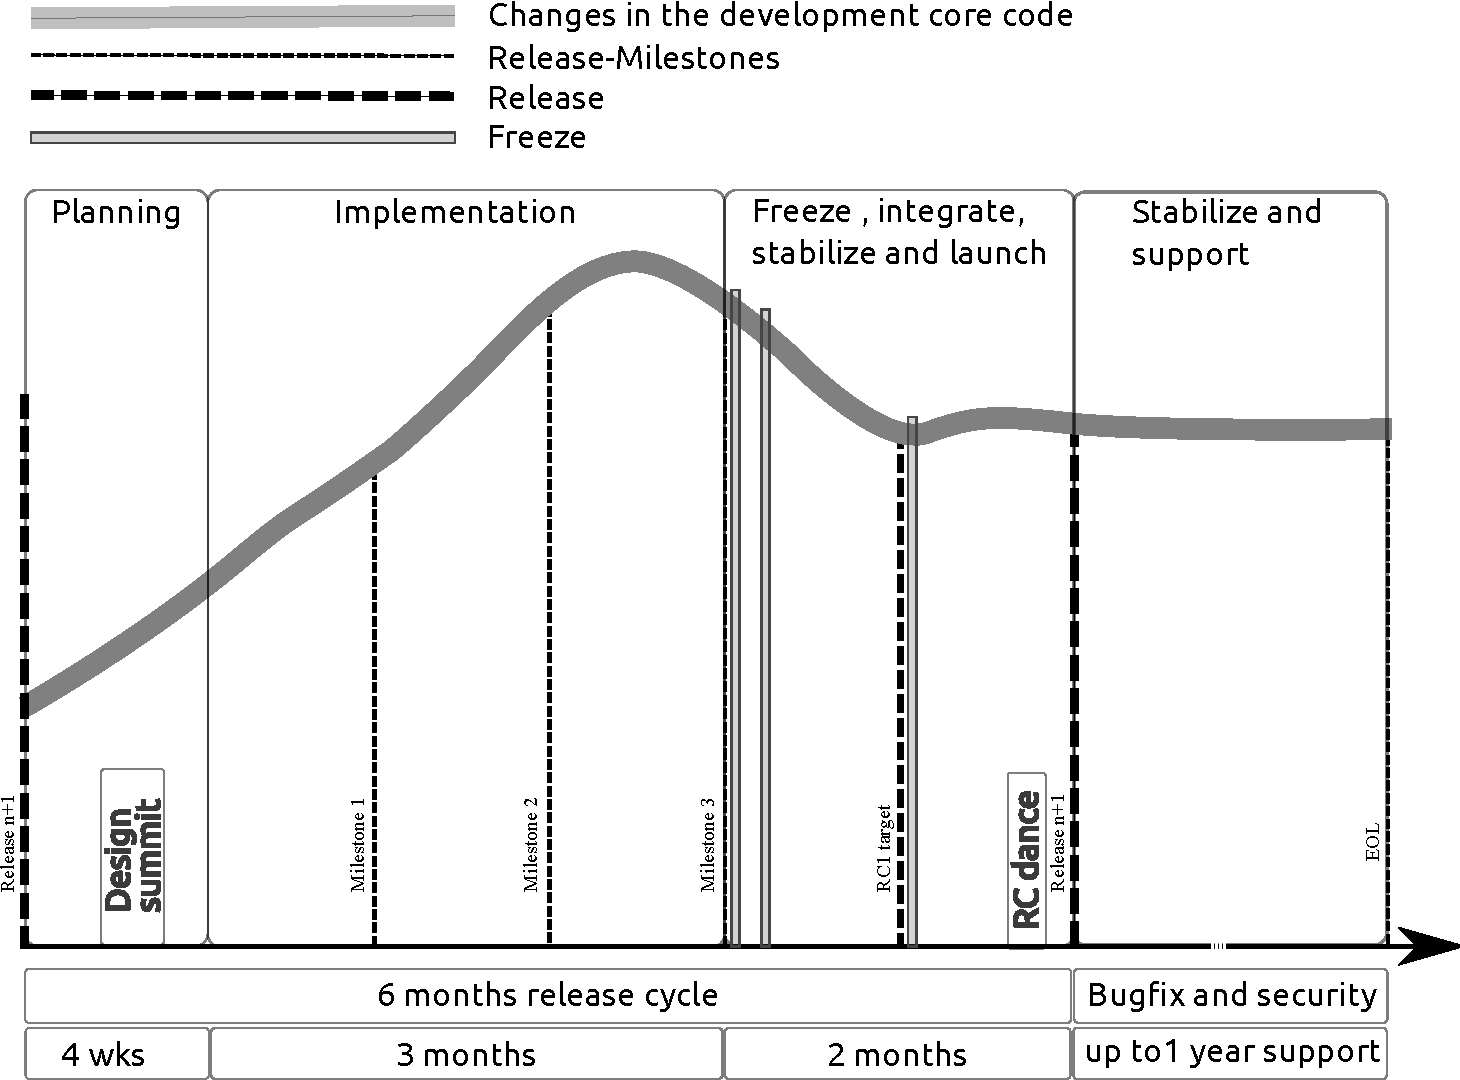
\includegraphics[keepaspectratio=true,width=0.9\textwidth]{release-management-overview.pdf}
  \caption{Overview of the OpenStack standard release cycle.}
 \label{fig:3stageprocesspic}
\end{figure}



The overall release management process, as illustrated in \Cref{fig:3stageprocesspic}, follows a plan, implement, freeze, stabilize and launch cycle between releases. Each release is then re-stabilized with \emph{a posteriori} release updates to fix bugs and security issues. Nevertheless, the process described so far is just the most recurrent pattern within OpenStack, the default \emph{modus operandi}. The described process is actually quite open and liberal. It acts as a recommendation for the different teams so that whatever is developed is then later more smoothly integrated, stabilized and released in a coordinated fashion. 

Since October 2016 (affecting the 'Newton' release), OpenStack actually recommends its project teams to choose from four different release management models: \emph{Common cycle with development milestones}, \emph{Common cycle with intermediary releases}, \emph{Trailing the common cycle} and \emph{Independent release model}.  
Most of these models follow a common six-month development cycle, some give intermediary releases within the six-months cycle and others are allowed to manage their own release strategy\footnote{See \url{http://docs.openstack.org/project-team-guide/release-management.html} for the details of each release management model.}.  

% these could actually be normal size to help reader
\begin{description}[leftmargin=!]
\footnotesize
\item[Common cycle with development milestones] The official and default time-based model followed by most teams. It results in a single release at the end of the development cycle and includes three development milestones (as in \Cref{fig:3stageprocesspic}).

\item[Common cycle with intermediary releases] For project teams wanting to do a formal release more often, but still wanting to coordinate a release at the end of the cycle from which to maintain a stable branch. Recommended for libraries and for more stable components, which add a limited set of new features and do not plan to go through large architectural changes.

\item[Trailing the common cycle]  For project teams that rely on the completeness of other components (e.g., packaging, translation, and UI testing) and may not publish their final release at the same time the other projects. For example, teams packaging and deploying OpenStack components need the final releases of many other components to be available before they can run their own final tests. Cycle-trailing project teams are given an extra two weeks after the official release date to request the publication of their own releases. They may otherwise use intermediary releases or development milestones. 

\item[Independent release model]  For project teams that do not benefit from a coordinated release or from stable branches. They may opt to follow a completely independent release model. Suitable for example for the OpenStack's own infrastructural systems (e.g., the ones supporting upstream testing and integration) as well for components with little dependence on the overall Openstack core architecture. 
\end{description}




\begin{quotation} 
\footnotesize
 ''We still have a coordinated release at the end of the six months for projects that are willing to adhere to those deadlines and milestones, but the main change is that we will move from managing most of them to refine processes and tools for each project to be able to produce those releases more easily. The development cycle will still be using a six months development cycle, even if some projects might do intermediary releases where it makes sense, but will still organize almost everything under a six months development cycle between design summits.`` --- Thierry Carrez , 15 May 2015\footnote{Transcribed from video, see [6:34--7:00] \url{https://www.openstack.org/summit/vancouver-2015/summit-videos/presentation/the-big-tent-a-look-at-the-new-openstack-projects-governance}.}
\end{quotation}



In an attempt to sum up and aggregate key elements of our narrative,  the timeline in \Cref{fig:process-timeline} highlights key events and turning points on the evolution of release management at OpenStack. From the first days, when the overall development was shaped by the official software development processes institutionalized  at NASA, then the spin-off as an open-source project with releases at every three months,  then the shift towards a more liberal release cycle of six months, and later,  after a period of much growth, the co-existence of multiple release models trailing a common six-month release cycle. 



\begin{figure}[!ht]
 
\centering


\newlength\yearposx
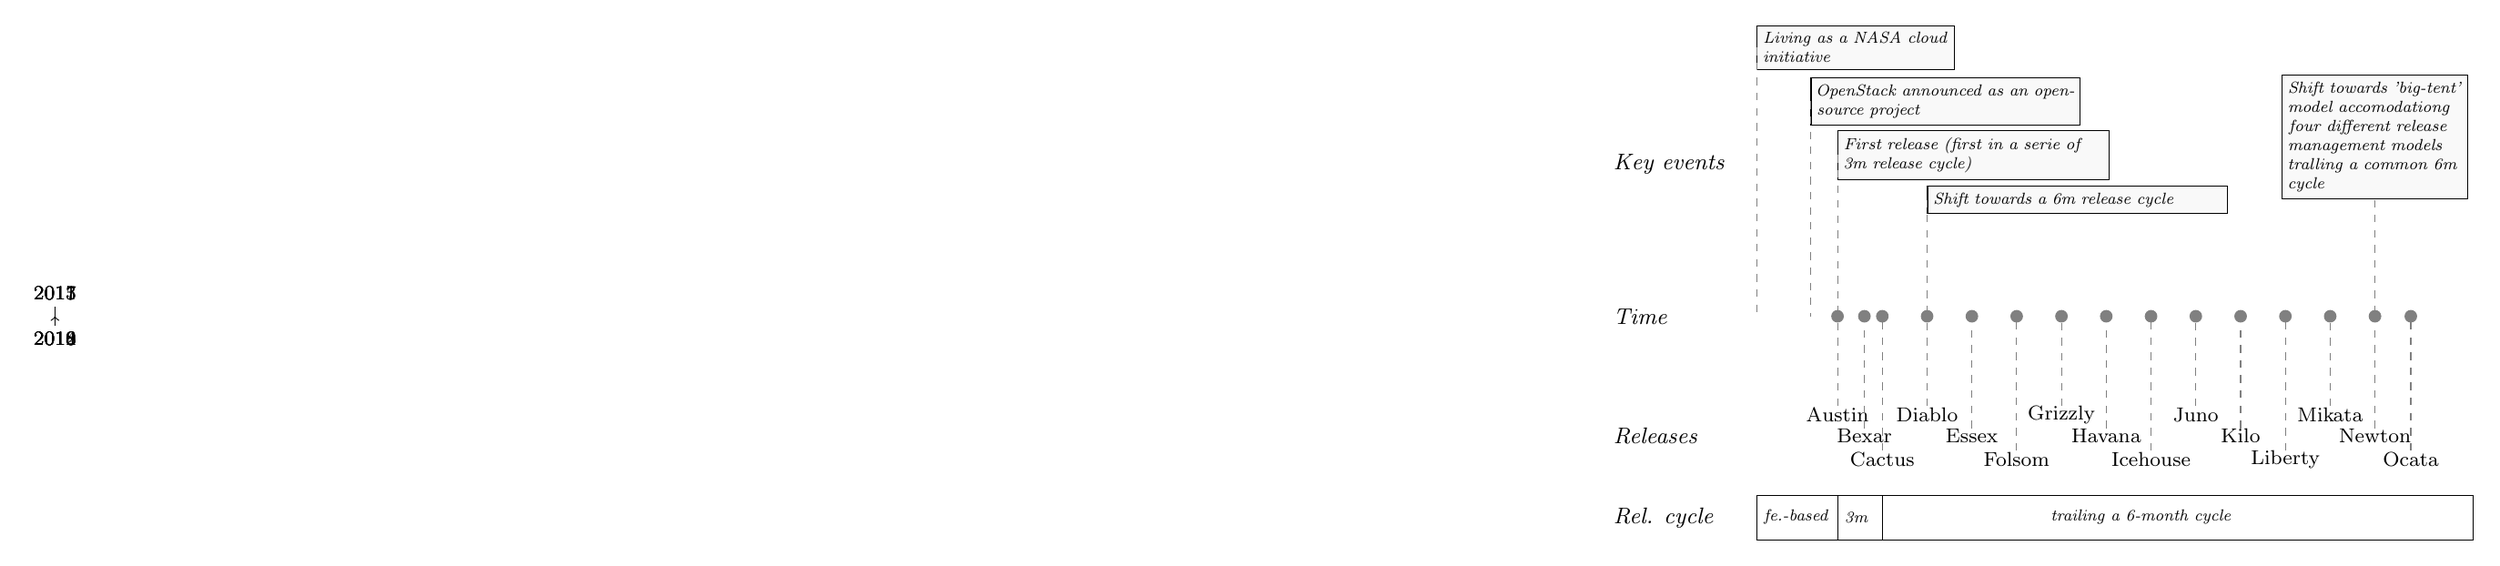
\begin{tikzpicture}[scale=1.25]
   

        \foreach \x in {2010,2011,2012,2013,2014,2015,2016,2017,2018}{
        \pgfmathsetlength\yearposx{(\x-1990)*1cm};
        \coordinate (y\x)   at (\yearposx,0);
        \coordinate (y\x t) at (\yearposx,+3pt);
        \coordinate (y\x b) at (\yearposx,-3pt);
    }
    

    


\begin{scope}[every node/.style={font=\small\itshape}]


\node at (2010-1990-1.7,1.7) [right] {\small Key events};

  
  

\node at (2010-1990-1.7,0) [right] {\small Time};


\node at (2010-1990-1.7,-1.33) [right] {\small Releases};




\node at (2010-1990-1.7,-2.25) [right] {\small Rel. cycle};

\end{scope}



  \node[scale=0.8, draw, align=left,fill=white!95!gray,text width=3.2cm, font=\itshape\footnotesize, right] at (2010-1990,3) 
  (EV1)   {Living as a NASA cloud initiative};

  \path[dashed] (2010-1990,3) edge [gray] (2010-1990,0);


  \node[scale=0.8,draw, align=left,fill=white!95!gray,text width=4.45cm, font=\itshape\footnotesize, right] at (2010.6-1990,2.4) 
  (EV1)   {OpenStack announced as an open-source project}; 
  
  \path[dashed] (2010.6-1990,2.4) edge [gray] (2010.6-1990,0);
    
    

  \node[scale=0.8,draw, align=left,fill=white!95!gray,text width=4.5cm, font=\itshape\footnotesize, right] at (2010.9-1990,1.8) 
  (EV1)   {First release (first in a serie of 3m release cycle)}; 
  
  \path[dashed] (2010.9-1990,1.8) edge [gray] (2010.9-1990,0);    

 
    

  \node[scale=0.8,draw, align=left,fill=white!95!gray,text width=5cm, font=\itshape\footnotesize, right] at (2011.9-1990,1.3) 
  (EV1)   {Shift towards a 6m release cycle}; 
  
  \path[dashed] (2011.9-1990,1.3) edge [gray] (2011.9-1990,0);    

 
 
 
  \node[scale=0.8,draw, align=left,fill=white!95!gray,text width=3cm, font=\itshape\footnotesize] at (2016.9-1990,2) 
  (EV1)   {Shift towards 'big-tent' model accomodationg four different release management models tralling a common 6m cycle}; 
  
  \path[dashed] (2016.9-1990,1.3) edge [gray] (2016.9-1990,0);    

  
  
  
  
        \draw [->] (y2010) -- (y2018);
       \foreach \x in {2010,2011,2012,2013,2014,2015,2016,2017,2018}
        \draw (y\x t) -- (y\x b);
 
     \foreach \x in {2010,2012,2014,2016,2018}
        \node at (y\x) [below=3pt] { {\footnotesize \x}};
    \foreach \x in {2011,2013,2015,2017}
        \node at (y\x) [above=3pt] {{\footnotesize \x}};
       
       
     \node at (2010.9-1990,-1.1) (A)  {\footnotesize Austin};
     \node at (2011.2-1990, -1.33) (B)  {\footnotesize  Bexar};
     \node at (2011.4-1990,-1.6) (C)  {\footnotesize  Cactus};
     \node at (2011.9-1990,-1.1) (D)  {\footnotesize  Diablo};
     \node at (2012.4-1990,-1.33) (E) {\footnotesize  Essex};
     \node at (2012.9-1990,-1.6) (F)  {\footnotesize Folsom};
     \node at (2013.4-1990,-1.1) (G)  {\footnotesize Grizzly};
     \node at (2013.9-1990,-1.33) (H)  {\footnotesize Havana};
     \node at (2014.4-1990,-1.6) (I)  {\footnotesize Icehouse};
     \node at (2014.9-1990,-1.1) (J)  {\footnotesize Juno};
     \node at (2015.4-1990,-1.33) (K) {\footnotesize Kilo};
     \node at (2015.9-1990,-1.6) (L)  {\footnotesize Liberty};
     \node at (2016.4-1990,-1.1) (M)  {\footnotesize Mikata};
     \node at (2016.9-1990,-1.33) (N)  {\footnotesize Newton};
     \node at (2017.3-1990,-1.6) (O)  {\footnotesize Ocata};


      
          \fill [gray] (2010.9-1990,0) circle (2pt);
     \path[dashed] (2010.9-1990,-1) edge [gray]  (2010.9-1990,0);s
      
          \fill [gray] (2011.2-1990,0) circle (2pt);
     \path[dashed] (2011.2-1990,-1.25) edge [gray] (2011.2-1990,0);
     
          \fill [gray] (2011.4-1990,0) circle (2pt);
     \path[dashed] (2011.4-1990,-1.5) edge [gray] (2011.4-1990,0);
     
          \fill [gray] (2011.9-1990,0) circle (2pt);
     \path[dashed] (2011.9-1990,-1.0) edge [gray] (2011.9-1990,0);
     
          \fill [gray] (2012.4-1990,0) circle (2pt);
     \path[dashed] (2012.4-1990,-1.25) edge [gray] (2012.4-1990,0);
     
     
          \fill [gray] (2012.9-1990,0) circle (2pt);
     \path[dashed] (2012.9-1990,-1.5) edge [gray] (2012.9-1990,0);
     
     
          \fill [gray] (2013.4-1990,0) circle (2pt);
     \path[dashed] (2013.4-1990,-1.0) edge [gray] (2013.4-1990,0);
     
          \fill [gray] (2013.9-1990,0) circle (2pt);
     \path[dashed] (2013.9-1990,-1.25) edge [gray] (2013.9-1990,0);
     
          \fill [gray] (2014.4-1990,0) circle (2pt);
     \path[dashed] (2014.4-1990,-1.5) edge [gray] (2014.4-1990,0);
     
       
          \fill [gray] (2014.9-1990,0) circle (2pt);
     \path[dashed] (2014.9-1990,-1.0) edge [gray] (2014.9-1990,0);
       
          \fill [gray] (2015.4-1990,0) circle (2pt);
     \path[dashed] (2015.4-1990,-1.25) edge [gray] (2015.4-1990,0);
     
     
          \fill [gray] (2015.9-1990,0) circle (2pt);
     \path[dashed] (2015.9-1990,-1.5) edge [gray] (2015.9-1990,0);
     
     
     
          \fill [gray] (2016.4-1990,0) circle (2pt);
     \path[dashed] (2016.4-1990,-1) edge [gray] (2016.4-1990,0);
     
     
          \fill [gray] (2016.9-1990,0) circle (2pt);
     \path[dashed] (2016.9-1990,-1.25) edge [gray] (2016.9-1990,0);
     
     
     
          \fill [gray] (2017.3-1990,0) circle (2pt);
     \path[dashed] (2017.3-1990,-1.5) edge [gray] (2017.3-1990,0);
     





\draw (2010-1990,-2) rectangle (2010.9-1990,-2.5) ;
\node at (2010-1990,-2.27) [scale=0.8,font=\itshape\footnotesize,, right, text height=3pt] {fe.-based};



\draw (2010.9-1990,-2) rectangle (2011.4-1990,-2.5);
\node at (2010.9-1990,-2.27) [scale=0.8,font=\itshape\footnotesize,, right, text height=3pt] {3m};



\draw (2011.4-1990,-2) rectangle (2018.0-1990,-2.5);
\node at (2013.2-1990,-2.27) [scale=0.8,font=\itshape\footnotesize, right, text height=3pt] {trailing a 6-month cycle};


\end{tikzpicture}
 
 

  \caption{OpenStack releases and key events shaping them.}
 \label{fig:process-timeline}
\end{figure}




\section{Results: a organizational view}
\label{sc:tools}




\begin{figure}[!ht]
 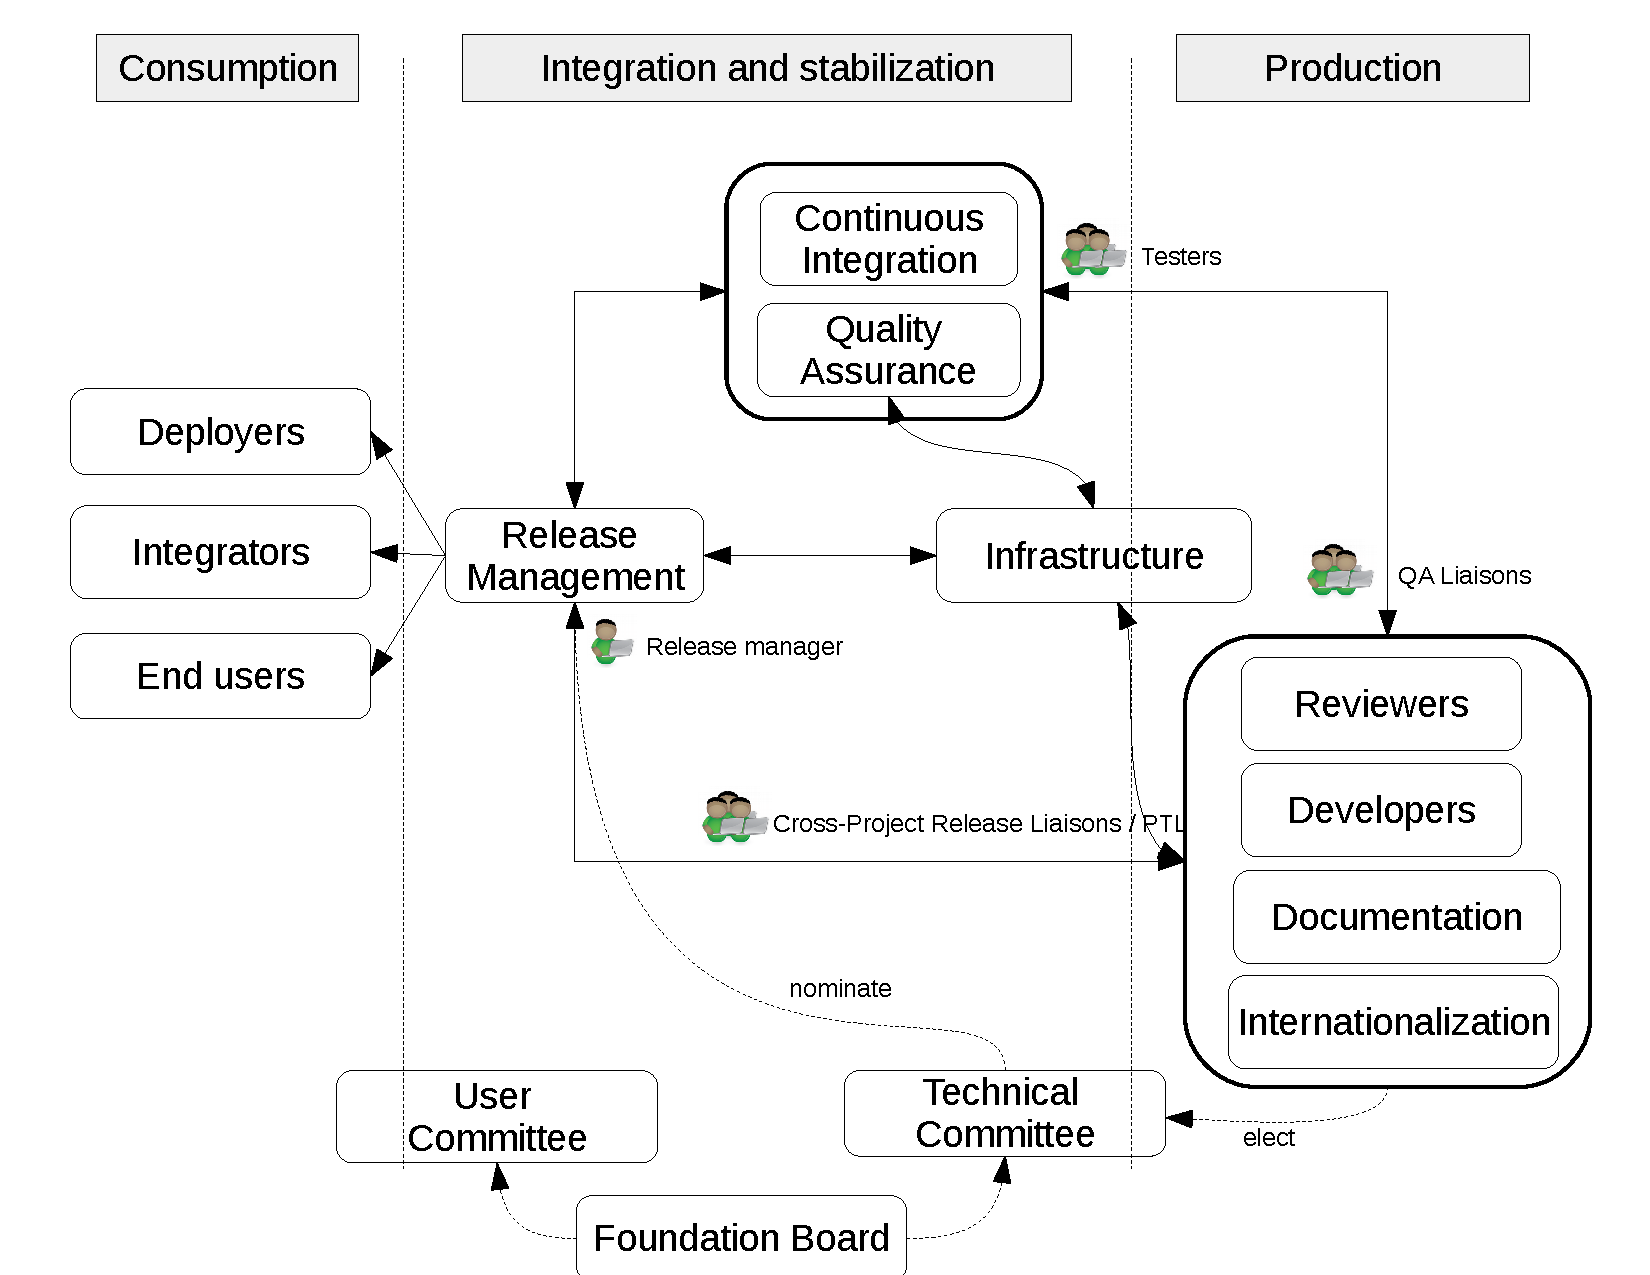
\includegraphics[keepaspectratio=true,width=0.9\textwidth]{./release-management-organization.pdf}
 % release-management-organization.pdf: 0x0 pixel, 300dpi, 0.00x0.00 cm, bb=
 \caption{organizational design supporting release management}
\end{figure}



\begin{newStuff}
 HERE I am deleting the tools section while drawing and discussing the organizational design 
 
 %%%%%%%% Prelude on the organiational side  
After offering a processual view on release management at OpenStack , we continue by addressing how the organizational design that supports it. We  organize our processual view from production side to the consumption. After all, the release management is very a wide process that impacts  multiple actors involved in the production and consumption of digital technologies. In our case release management impacts the ones incrementally developing the multiples pieces of OpenStack (e.g., software developers), the ones integrating and stabilizing such pieces (e.g., testers) as well as the ones marketing, communicating and using the new releases. 

\subsection{Organizing incremental product development}

%%% Oversea leaders  


Before detailing the release management practices of different actors across the OpenStack production ecosystems, we must address the overall OpenStack governance. As many other large contemporary digital ecosystems (e.g., Linux, Android, Apache, Mozilla, Eclipse, and R among others, OpenStack is governed by a nonprofit non-stock foundation. The OpenStack fondation is funded by members. Such members can then elect the board of directors. Such board of directors are rarely involved in release management issues, they rarely interfere directly in production issues and focus on startegic and finantiaal issues (e.g., where the money raised by the memberships should spent.) Production issues are handled mostly by the \ac{TC} that is elected every six-months by active contributors to the project. The \ac{TC} have a person employed dirctely by the OpenStack Foundation (note not employed by companies contributing to the project) that overseas the overall release management practices at OpenStack known as the 'release manager'. The release manager, as an elected member of the \ac{TC} can bring unsolved issues to the  Board for voting.  While the \ac{TC} deals most with production issues, the  \ac{User Committee} deals more with consumption issues. Even if not directly involed in release software, they should provide requirements and guidance on what should be releases as well provide feedback on the deployment different OpenStsck releases. Given that \ac{User Committee} is more interested on what is released than how it is released, the v\ac{User Committee} have little influence on the release management pracices of OpenStack. To sum up, besides pontual coordination with the board of directors and the  User Committee, the \ac{TC} is the main body steering release management at OpenStack.  

%%%%  Production
%%%%  Sub-projects developing functionalities (aka features) %%%% 

Both in the production and in the consumstion side, OpenStack is a complex moving target. In one hand every minute dozens of atomic patches (aka contributions) are submitted by developers that are later reviewed, tested, and integrated within OpenStack as a whole prior to a formal release. On the other hand, OpenStack is deployed across thousands of data-centers worldwide at very fast pace. Many consumers (the ones using, deploying or integrating ) 
The product development is organized across the different  sub-project teams. They are the ones developing functionalities (aka features) and they are responsable for maintaining their on code-repository. 

Contrasting with many software development projects, the source-code is not orchestrated by a single software repository. Instead, the source code is orchestrated across multiple software repositories (to achieve higher modularity), each managed by its own sub-project teams. During the first year of OpenStack, and as in many other software development projects,   a selection of core and mature repositories at a given time dictated what was in the official OpenStack release. This is called the \textit{integrated release model}. Since the OpenStack Liberty release (October 2015), tags signed by the  \ac{TC}  dictate what is the official OpenStack release. This is called the \textit{big tent release model}. In other words, since the Liberty release, OpenStack software releases are not seen as a selection of core repositories, but as code tagged by the  \ac{TC} across all the repositories of OpenStack. It is important to note that only software officially released by OpenStack can use the OpenStack trademarks, for example, for marketing the software using the OpenStack name or logo\footnote{See the guidelines laid out in sections 4.1 and 4.13 of the OpenStack Foundation Bylaws for legal details at \url{https://www.openstack.org/legal/}.}.  

Here we identify a challenge, pertainign the ecosystems boundaries. One technologies releatively simple and developed by a single firm, there is a awareness of the boundaries of the system (who develpåes and what was developed), but in more reaas. In the case of OpenStack, the boundaiies of the product development become blury, no single person or organizatinan could have a clear view of what should be included in the next releaase. This is not surprising, as thounsands of developers and hundreds of copanies recurrently add new functioaly to the systems.  

At its more mature phase, 

.  At this planning stage, developers gradually leave the \textit{integration} and \textit{stabilization} mode to enter again into the \textit{planning} and \textit{development} mode. Besides considering what should be done, sub-project teams concerned with with release management should also consider what can be done on time to be included in the upcoming release. They are free to work on more disruptive changes that will integrated later, however as OpenStack is an always evolving target, the later changes are integrated with the official code-base the more changeling the integration will be.   In this sense release management discourages disruptive changes, entropy and possibly innovation. The ones that pursue disruptive changes will be challenged by the release management proce
ss.

At the planning stage  partially overlaps with the OpenStack design summit, many of the discussions take place face-to-face.  The OpenStack 
 infrastructure team provides  tools that facilitate the discussion and formalization of what should be developed during the next milestones.
 At this stage, the sub-projects teams should be developing blueprints, specifications and  task plans.  But, developers might paying attention with bugs that in meanwhile where found in the last release. 
 
Sub-projects are responsable and control their own code-repository. There are also responsable for intependintly electing a PTL 

The Release Management Liaison is responsible for communication with the Release Management team. Its tasks are described in the project team guide: http://docs.openstack.org/project-team-guide/release-management.html . That task has been traditionally filled by the PTL, but they may now delegate this task if they wish.

    By default, the liaison will be the PTL.
    The liaison may further delegate work to other subject matter experts


OpenStack have an official procedure for the sub-project initiations to grant the release management to publish releases from their sub-project and connect to the Continous Integration, Testing and and peer-review systems.
\footnote{See \url{https://docs.openstack.org/infra/manual/creators.html}} 


Note also that 
Inter-project Liaisons

''In some cases, it is useful to have liaisons between projects. For example, it is useful for the Nova and Neutron projects to have liaisons, because the projects have complex interactions and dependencies. Ideally, a cross-project effort should have two members, one from each project, to facilitate communication and knowledge transfer.'' \footnote{See \url{https://wiki.openstack.org/wiki/CrossProjectLiaisons}}.


%% Then there is the Internationalization (I18n) team 

''To make OpenStack ubiquitously accessible to people of all language backgrounds.``\footnote{See \url{https://governance.openstack.org/tc/reference/projects/i18n.html}.}


%%%% There is also the 
''provides guidance, assistance, tooling, and style guides enabling OpenStack project teams to produce consistent, accurate, and high-quality documentation``\footnote{See https://governance.openstack.org/tc/reference/projects/documentation.html}.



%%%% Infrastructure team 

Infrastructure team 
These include tools for version and revision control, continuous integration, testing, and code-reviewing. 
communication, coordination, and collaboration tools that are used 

''Develop and maintain the tooling and infrastructure needed to support the development process and general operation of the OpenStack project.`` \footnote{See https://governance.openstack.org/tc/reference/projects/infrastructure.html}.



%%% Quality Assurance Team 

''Develop, maintain, and initiate tools and plans to ensure the upstream stability and quality of OpenStack, and its release readiness at any point during the release cycle.``\footnote{See \url{https://governance.openstack.org/tc/reference/projects/quality-assurance.html}}





%%% Midlde release managemnt team 

''Coordinating the release of OpenStack deliverables, by defining the overall development cycle, release models, publication processes, versioning rules and tools, then enabling project teams to produce their own releases.``\footnote{See \url{https://governance.openstack.org/tc/reference/projects/release-management.html}.}




Develop tools together with the infrastructure team to automate the release management process
Applies tags on the sub-project  

The release management team, sends annoucements, \citep{PooCaamanoKnauss_et_al2017}, and request decision on whats is and whats is not release to the project team leaders. 

According to Poo-Caamano  \citep{PooCaamanoKnauss_et_al2017} that investigated communication in release management coordination at OpenStack, 
, a common infrastructure is required to facilitate communication and coordidantion among the  release management team and the different sub-projects. Asynchronous channels, such as mailing lists, are preferred as they act as an egalitarian media for discussion among a wide range of participants as the messages can be archived and made searchable. Furthermore they do not exclude participants that cannot attend a physical face-to-face discussion and are preferred by developers that may not be as fluent as their native English-speaking team mates \citep{PooCaamanoKnauss_et_al2017}. 






%%% Concuption side 
It's not a download of project. But a subset of projects. Deployed consume different pieces and in a different way. 




 
 
\end{newStuff}


\begin{newStuff}
 HERE are the links and boxes that the diagram must  have: 

  LEFT: Testing, CI, Review, Infrastructure 
   MIDLE: Cross release management team, PTL, BOARD, release management team 
 RIGTT SIDE: End-users, Deployers , Other projects integrating with OpenStack.  


  LINK TOOLS -> Infrastucture, RM on tools 
  LINK communication, coordination, and collaboration tools  sub-projects.
 
\end{newStuff}


\begin{newStuff}




\begin{newStuff}
TODO ADD to Theoretical background,  release encompasses  meeting a number. 
the Semantic Versioning Specification (SemVer) adopted by OpenStack that distinguishes between MAJOR, MINOR and PATCH increments.. The use of tags allows both developers and users of OpenStack to track the incremental evolution of the software being developed intuitively. Naming different versions of the software is essential for both developers and users of OpenStack that often need to deal with multiple versions of OpenStack. 


 
 

\end{newStuff}






 
 
\subsection{Reliance on a infrastructure connecting developers, reviewers} 

Release management includes deciding if a certain piece of code is ready to be released or not. In other words, stakeholders in the release management must ensure whether the quality of certain software is at an acceptable level for release. Therefore, release management and peer review are inseparable processes 
\citep[]{Jrgensen2001,SharmaSugumaran_et_al2002,NarayanFinis_et_al2012,StarkOman_et_al1999}. Many successful open source software projects employ formal code review activities prior to the release \citep{Michlmayr2007}. Core reviews are effective means for quality assurance, knowledge dissemination, social relationship building, achieving better designs, and ensuring maintainable code in long term \citep{BosuCarver_et_al2017}. In the OpenStack case, peer review is handled by Gerrit\footnote{See \url {https://www.gerritcodereview.com/} for more information on Gerrit.}, a insfratrural tool that hides many of the complexities of reviewing code. That infrastructural tool connects the QA, CI, the developers submiting changes, the developers reviewing changes. The process is quite straightforward: developers implement new features and submited then to Gerrit.  Then the systems from the CI team attemnts the build and tests agains the overal software as a whole. Every change will get votes (votes from the robta ) They can give postive and negative votes. 
All this takes place in a sequence towards the future landing of the code and its later release. 

% H: Code review frequesncy icnreases closer to the releases 

% H: Code review entromy changes close to the releases 


Release management constrains the code review processes.  A change should be proposed a few weeks before the targeted milestone publication date in order to be reviewed in time and included in the same milestone. Furthermore, the use of release management freezes purposively minimizes the time that code reviewers spend 'drowned' in late code reviews for features proposed late. After the freezes, new feature code reviews should be rejected by the review team and postponed until the next series development opens. In order for the teams to integrate, stabilize and launch what was implemented so far, code review efforts should be limited to existing code and bug fixing submissions. Features implemented late can introduce regression bugs close to the release date, undermining the quality of OpenStack software as a whole. 


While code reviews lead to human judgments on what code is ready to be released or not, the Quality Assurance (QA) and the Continuous Integration (CI) operations produce semi-automated judgments on whether a piece of code is of sufficient quality be released or not.  The mission of Quality Assurance is to ``develop, maintain, and initiate tools and plans to ensure the upstream stability and quality of OpenStack, and its release readiness at any point during the release cycle''\footnote{See \url{http://wiki.openstack.org/wiki/QA} for the mission statement of the OpenStack Quality Assurance team.}. This mission underlines the importance of automation in complex software development settings:


Test results are reported to Gerrit by Zuul in the form of a 'machine' vote that will complement the human code-reviews. Only after the code reviews have been completed and the code passed the Jenkins/Zuul tests, the 'gate opens' and the code can finally 'land' into the official master branch. A stable branch will be cut by the end of the release cycle from this master branch.  

 The release manager job here is the only changes evaltuated with positive votes will be released. 


As fixing bugs requires much cooperation and coordination among different teams.  As pinpointed by Poo-Caama{\~{n}}o et al. (2017)  \citep{PooCaamanoKnauss_et_al2017}, release management information should be communicated across and made available to the overall ecosystem participants. 

While the code reviews orchestrated by Gerrit provide individual formative feedback on the code-contributions, the continuous integration tests run by Jenkins  and Zuul provide machine-made (aka testing bots) summative feedback of the code contributions. Armisen et al. (2016) \citep{armisen2016formative} studied the the interplay between formative and summative feedback at OpenStack. They suggest that summative feedback (i.e., testing bots) influences how developers take formative feedback (i.e., code reviews). 

While a code review vote is highly personal and might vary from reviewer to reviewer, the automated testing results are more often unassailable. In an analogy with the academic world, we could say that code that does not pass the continuous integration tests is code that tends to be "desk rejected". While code contributions are reviewed once in Gerrit, both Jenkins and Zuul run the automated tests twice, before and after the approval by the reviewers.  The OpenStack community claims that continuous integrations tests are in line with the open and egalitarian nature of the OpenStack project as, after all, it should not matter where the code comes from, from which particular developer or company, it  needs to pass the same tests to make it to the official code base. At this point competitive tenstion betwoo TODO 

\begin{quotation} 
\footnotesize

``OpenStack projects do not permit anyone to directly merge code to a source code repository. Instead, any member of a core reviewer team may approve a change for inclusion, but the actual process of merging is completely automated. After approval, a change is automatically run through tests again, and only if the change passes all of the tests, is it merged.

This process ensures that the main branch of development is always working (at least as well as can be determined by its testing infrastructure). This means that a developer can, at any point, check out a copy of the repository and begin work on it without worrying about whether it actually functions.

This is also an important part of the egalitarian structure of our community. With no member of the project able to override the results of the automated test system, no one is tempted to merge a change on their own authority under the perhaps mistaken impression that they know better than the test system whether a change functions correctly.''
--- OpenStack Project Team Guide, as last edited on 20 Sep 2017\footnote{See \url{https://docs.openstack.org/project-team-guide/testing.html}}.

\end{quotation}

 
 





% Eija has edited up to here on 28082918. Will continue tomorrow morning

\subsection{Cross-team release management } 

The release management team filters, assesses, validates and releases the overall code base. The team manages the release process for the many deliverables proposed by each project team at a given development cycle. The team also provides and maintains the many tools that support the overall release management duties (e.g., the Reno release notes manager\footnote{See \url{https://docs.openstack.org/reno} for details.}). The release management team acts as a cross-project organization that spans the different project teams. It relies on a liaison from each team project to help with coordination and release-related tasks. This release management liaison is often the Project Team Leader or someone formally designated by the Leader. Release management liaison should exhibit leadership especially within the project team, exhibit communication skills within and across teams, follow the release guidelines, keep track of the development cycle tasks, attend the cross-project meetings (e.g., the  \ac{TC} meetings that generally happen on Tuesdays) and ensure that known bugs are correctly reported and triaged. Release management liaisons need to deal with many of the interdependencies across the different OpenStack project teams and their repositories.

In this way, much of the work with release management remains largely manual, far from fully automated. The release management team develops and maintains a significant number tools and scripts to handle the release process, but much of the work remains manual, something that the OpenStack community acknowledges and intends to  automate further. Since the release of the Liberty series (12th release of the project on 16 October 2015),

Using the devops. 


Release Liasons 

TODO Add the 7 duties of the release liasons
https://docs.openstack.org/project-team-guide/release-management.html




\iftoggle{showOrgDescription}{
\subsection{Release management at OpenStack - organizational design supporting it}


\todo{Check this is congruent with \url{https://docs.openstack.org/project-team-guide/release-management.html} }


``Each project team should designate a stable branch cross-project liaison as the main point of contact for all stable branch support issues in the team. If nobody is specifically designated, the PTL will be assumed to cover that duty'' \url{https://docs.openstack.org/project-team-guide/stable-branches.html#support-phases}



``o Gerrit should be reviewed and seconded by two project-specific stable maintenance team members before it is approved. Where a team member has backported a fix, a single other +2 is sufficient for approval.'' \url{https://docs.openstack.org/project-team-guide/stable-branches.html#support-phases} 


\begin{itemize}
 \item Release management team 
 \item Cross project liason 
 \item Infrastructure team 
 \item QA team
 \item PTL 
 \item Technical Committee (TC)
\end{itemize}


Such tags rely on GPG 

``For other changes within an existing project team, like addition of a new git
repository or self-assertion of a tag, we use lazy consensus. If there is no
objection posted one week after the change is proposed (or a significant new
revision of the change is posted), then the change can be approved by the
chair.

One exception to this would be significant team mission statement changes,
which should be approved by a formal vote after an in-meeting discussion.

In corner cases where the change is time-sensitive (like a deliverable
reorganization which blocks a release request), the chair may fast-track the
change, but should report on that exception at the next TC meeting.
''

\url{https://git.openstack.org/cgit/openstack/governance/tree/reference/house-rules.rst}




As in http://git.openstack.org/cgit/openstack/releases/tree/README.rst

Who is Responsible for the Release?
===================================

The release team is responsible for helping to clearly signal the
nature of the changes in the release through good version number
selection.

The project team is responsible for understanding the implications for
consuming projects when a new release is made, and ensuring that
releases do not break other projects. When breaks occur, the project
team is responsible for taking the necessary corrective action.
}
{}


\section{Discussion}





\begin{newStuff}
 TODO integrate the design from ISJ \citep{SharmaSugumaran_et_al2002} 
 
Release management: a core group member volunteers to serve as the release manager
as the project nears a product release. The release manager identifies outstanding problems
and  their  solutions  and  makes  suggested  changes. The  role  of  release  manager  is  rotated
among the members of  the core group.


``refers to the concept of a “release train”''\citep{KhomhAdams_et_al2015}




Mozilla realized that there was a “lack of a single team or person driving the release process for each release”. By creating a dedicated release management team for this task, they were able to overcome this problem. \citep{KhomhAdams_et_al2015}



Table with problems that justify such design 
\begin{table}[H]
\begin{tabular} {lll}
Problem & Organizational Fix & Implementation\\
Fuzziness of the boundaries & Adoption of the big-tent  & Liberty release\\
Coordination & Design summit, Introduction of the release liaison, communication infrastructure & ? \\ 
Who is responsable for the releases & Release manager Therry & ? \\ 
Not sufficient time for introducitn & ChaNGE FROM 3MONTHS O 6 MONTH & ? \\ 
dIFFENRE SUB-PROJECT TEAM have different releases & & \\ 
tESTING, TRANSLATION AND DOCUEMETNTIN  amoving target & feature freezes &  ? \\ 
Planning & Involve developers at the design summit, infra
 for dissusxcion & ? \\ 
 Meritocracy, Conflict of interest & Creation of a foundation, Elections of PTL, TC and &  release manager employd   \\  
\end{tabular}
\end{table}




\end{newStuff}


\subsection{Current problems}




- Nobody is listening 
- Discoraging potential contributors 
- Feed back from operators 

Devs are from Venus, Ops are from Mars” – Steven Haines 

\end{newStuff}









In this paper, we investigated release management at OpenStack while paying special attention to the overall process and the organizational design supporting it. Our findings complement the current body of empirical knowledge addressing release management in the context of open source software \citep{MichlmayrFitzgerald_et_al2015,PooCaamanoKnauss_et_al2017}. As release management practices are connected to other software engineering practices such as `planning, code-reviewing, continuous integration, quality assurance, documentation and translation, our results might connect with other issues of interest in the Software Engineering and Free/libre/open source (FLOSS) research communities. 

Prior work has already inquired on OpenStack release management issues (see \citep[pp 10-11]{Teixeira_et_al2015} for work bringing up collaboration issues and \citep[pp 80-82]{PooCaamano2016} for work pointing out communication issues). However, and to the best of our knowledge, this is the first paper paper that explicitly aims at describing how a large and complex open source software ecosystem refined its release model over time. We longitudinally followed OpenStack technology from its inception at NASA to its bootstrap as an open source project and its more mature phase characterized by a liberal time-based release strategy where multiple cycles co-exist.




When integrating with prior related literature, our results confirm the pivotal role of freezes within the release management process (cf. \citep{Fitzgerald2011,AnandBhatt_et_al2017}).
The use of the three freeze mechanisms by the release management team (i.e., “FeatureFreeze”, “SoftStringFreeze”,  and “HardStringFreeze”) encourages developers to progressively change their production focus from new developments to integration and stabilization of that what was developed so far (see \cref{t:3freezes}). 
In our case, the use of freezes forces developers that want to see their work in the next release to make three major shifts in the focus of the production: (1)  from the individual component level to the overall integration as a whole, (2) from developing new features to ensuring their landing, integration and stabilization, and (3) from individual work, or collaboration within smaller teams, to coordination across the overall community. Our investigation found the use of freezes particularly helpful for the practice of user-interface testing automation (see \Cref{sc:tools} for a short account on the efforts of the Horizon project team to automate the testing of dynamic HTML user interfaces). 





Also, in the light of prior work, the  release management process of OpenStack can be considered a hybrid of feature-based and time-based release management \citep[pp 23]{Wright2012}. In addition to regular releases every six months, OpenStack also attempts to introduce new features at each regular release. At the planning stage, leaders of each project team choose a set of features  for the  next release. However, if these features are not stable enough to be included in the upcoming release, they will be left out by the cross-project release management team. 

As pointed out recently, release management constrains the evolution of the integrated whole  \citep[pp 4]{PooCaamano2016}.
 
 




By investigating both the release management processes and the tools that support it at OpenStack, we found both the micro-tagging approach and the Reno release notes manager as novel and distinctive from other open source release management cases \citep[c.f.,][]{MichlmayrFitzgerald_et_al2015,PooCaamanoKnauss_et_al2017}. Future research could report on how the OpenStack  \ac{TC} and the release management team employ repository tags to signal that a certain component of OpenStack was release managed (an indicator of quality), that certain component can be marketed as a core component of OpenStack, or that a given project followed a suitable design or achieved a high level of diversity in the affiliation of contributors (an indicator of a healthy collaborative project).  Assuming that others might be interested in Reno as a novel open source tool supporting release management processes, future research should explore whether the following characteristics of Reno could bring value to the practices of release management in particular and software engineering in general. 

\begin{itemize}
 \item Release notes are automatically associated with the release version based on the repository tags applied to the repository. It is not necessary to track changes manually outside the repository (e.g., in a bug tracker, a spreadsheet or other tool).
 \item Release notes are encoded within the source code repository at the side of correspondent features source code. This means that release notes can be written when the code changes within the same development environment.
 \item Release notes go through the same review process used for managing code and other documentation changes.
 \item Release notes are encoded in a standardized format. Notes are organized into logical groups based on whether they describe new features, bug fixes, known issues, or other topics of interest to deployers, users, and developers. 
 \item Prior to delivering new features to the release management team, release notes can be automatically aggregated and documented from the source code repository with Reno.  Developers only need to run a script that invokes Reno. 
\item Release notes can be easily located by project, release series, branch, earliest revision, and date, among other parameters.  Developers can search for specific sets of release notes and sections. 
\end{itemize}

Adding to prior work, and in addition to considering the overall release management process of OpenStack as a hybrid of feature-based and time-based release management, we also consider it as quite liberal. We found the OpenStack release management process to be liberal in multiple aspects: 
\begin{itemize}
 \item Liberal as the official releases dates, the milestones, and the freezes are not strict but negotiated and applied by the release management team in cooperation with the different project teams. In an analogy with trains, a given train might be scheduled to depart at a given time, nevertheless, they might come a bit before or a bit later due to a number of organizational or technical issues. Still, the train schedules remain a useful artifact for planning purposes. 
 \item Liberal as different teams (e.g., testing, drivers, documentation, and translation) are granted with extra days, or even a few weeks, to deliver their own releases. Releasing depends on the context, nature and interdependencies of the artifacts being developed. Examples include testing how a certain hardware driver complies with new developments, developing a new library that relies on external APIs and translating recent documentation to another language. 
\item Liberal as feature freeze exceptions are granted by the release management team and the \ac{TC} in exceptional cases (e.g., for landing a release critical fix).  These feature freeze exceptions need to be properly discussed and documented before being granted, controlled and monitored. 

\item Liberal, as well, as OpenStack started more recently recommending four different release management models. Even if most of the models trail the common six-month release 'train', the OpenStack governance recognized over time the need for certain teams and individuals to manage their own release strategy independently. 

\end{itemize} 


\begin{newStuff}
 ``The release team simplified its processes by establishing several standard release models for teams to follow. The models describe aspects of the release such as how version numbers are selected and the timing for producing artifacts during our regular cycle.`` \footnote{See \url{https://doughellmann.com/blog/2017/08/24/stop-working-so-hard-scaling-open-source-community-practices/}.}
\end{newStuff}



Given the complexity of the OpenStack software ecosystem in general and the historical evolution of its release management processes in particular, we opted to keep our main research efforts as descriptive. Our main contribution is then a straightforward longitudinal account of the release management practices at OpenStack, an account that, to our belief,  can bring issues of interests to the Software Engineering and Free/libre/open source (FLOSS) research communities. Both academics and practitioners can now assess the similarity or dissimilarity of the release management processual patterns of OpenStack with other projects - this kind of comparison can lead to lessons learned or even to improvements on the way organizations release software.  

We have studied, gained understanding and described many of the release management processes and tools with OpenStack. We have given our own interpretations of the release management phenomena in the context of OpenStack, that is, in an open source software ecosystem that has so far continuously grow in size and complexity. Our most striking finding is that the evolution of release management processes at OpenStack  has led to the co-existance of not one but several release management cycles. Since October 2016, the OpenStack release management formally recognize four different release management models. 

We can conclude that as a software ecosystem grows in size and complexity, its developers might follow not one but several release management cycles. This conclusion calls for further research investigating why, how, and when projects should implement multi-cycle release management strategies. In the particular case of OpenStack, it remains unexplored whether the formal co-existence of four different release management models has had a positive impact on the amount or quality of the software being contributed by its developers. Future research addressing multi-cycle release management strategies might be a fruitful avenue in Software Engineering. So far, we know that smaller open source projects at early stages traditionally announce releases once new features are implemented. We also know that large and successful open source projects benefited with the implementation of time-based release schedules \citep{MichlmayrFitzgerald_et_al2015}, but so far little is known about projects where multiple release models co-exist with each other as we found in our case. Future quantitative investigation unveiling causal relationships between the socio-technical characteristics of teams and artifacts (e.g., sub-projects team size, application vs. library, modularity, and coupling among many other socio-technical characteristics) and the different release management models, are,  in our view, research efforts worth being explored.                                                                                                                                                                                                                                                                                                                                                                                                                                                                                                                                                                                                                                                                                                                                                                                                                                                                                                                                                                                                                                                                                                                                                                                                                                                                                                                                                                                                                                                                                                                                                                                                                                                                                                                                                                                                                                                                                                                                                                                                                                                                                                                              
 







At this point, we are not attempting to evaluate, appraise or compare the captured release management processes of OpenStack. Our focus was on describing the most salient release management patterns by deeply studying them. Besides leading to descriptive findings, our investigation of OpenStack opens multiple avenues for future research. 

An obvious step is to move from a single case to a multipl case study design. Future research could analyze and juxtapose the processual practices of release management across multiple cases \citep{MichlmayrFitzgerald_et_al2015,PooCaamano2016}. Both within OpenStack, or in other projects, digital trace data generated by the upstream integration processes, the source code repositories, the code review systems, and the bug trackers could be used to triangulate the authenticity of the conceptual release management models in practice. \footnote{See \citep{HowisonWiggins_et_al2012,HedmanSrinivasan_et_al2013,Freelon2014,RuthsPfeffer2014,Crowston2017} 
for recent discussions on validity issues regarding the collection and analysis of digital trace data.} 
Also, it remains unknown why and how multiple release cycles co-exist in large and complex software ecosystems. Another salient issue pertains to the management of information regarding release management (e.g., should release management notes be stored at the side of the source code in the repository, or should new systems be developed for better structuring all information regarding release management).

Given the co-existence of multiple avenues for future research, and as we intend to continue our engagement with the OpenStack community, we plan to address some of the current challenges faced by the OpenStack release management team. The OpenStack community could benefit from better co-release practices with its end users and deployers, because their feedback often comes too late to shape the next immediate release cycle. Better practices could also reduce the large cognitive load that first time, part time and occasional contributors face releasing their software, because release management adds a set of discouraging barriers for contributors that are not that familiar with the overall research management processes.  Engaged empirical research taking a critical stance on these practical issues could lead to improvements in the release management process and overall organizational design of the OpenStack ecosystems.\begin{newStuff}While so far we had focused on processes and tools, future research should also explore the organizational design supporting and shaping release management at OpenStack. Along these lines, future research could engage with theoretical frameworks such as the Conway's mirroring hypothesis \citep{KwanCataldo_et_al2012}, socio-technical congruence \citep{CataldoHerbsleb_et_al2008} or socio-materiality \citep{OrlikowskiScott2008} to explore release management from an entangled organizational and technical perspective. After all, it is expected that the organizational design supporting release management is shaped by the artifacts being developed (e.g., code and documentation) and the other way around. The use of such theoretical frameworks challenges researchers to not separate organizational and technical issues from each other but build knowledge while intertwining them.                                                                                                                                                                                                                                                                                                                                                                                                                                                                                                                                                                                                                                                                                                                                                                                                                                                                                                                                                                                                                                                                                                                                                                                                                                                                                                                                                                                                                                                                                                                                                                                                                                                                                                                                                                                                                                                                                                                                    \end{newStuff}



  




















\section{Conclusions}


OpenStack implemented a time-based release strategy that trails a six-month cycle. Each cycle comprehends a planning stage, an implementation stage and freeze, stabilize and launch stage.
In the middle of each release cycle, the community relies on three freezes (i.e., “FeatureFreeze”, “SoftStringFreeze” and “HardStringFreeze”) that encourage developers to change their production focus from the development of components to the overall upstream integration and stabilization of components as a whole. This change affects much the work and communication patterns of the community. The implemented release management process exhibits hybrid characteristics of both feature-based and time-based release management strategies as the process is both feature and time oriented. Moreover, the implemented release cycle is quite liberal and in this way open to changes and flexible to adaptation. In particular contexts, different project teams across the community are allowed to work around the default six months release cycle. Even when the project advocates a six month release cycle, different release cycles do co-exist across the different OpenStack sub-projects.

The implementation of a liberal time-based release strategy is a complex process that intertwines with many other software development processes. In the case of large and complex open source software ecosystems, this requires the support of a well suited organizational design as much coordination is needed. Moreover, the process constrains the evolution of the integrated core and depends heavily on many software tools that make it possible. These tools help, for example, version control, revision control, continuous upstream integration, continuous upstream testing, and configuration management. Besides its acknowledged benefits (see \citep{MichlmayrFitzgerald2012}), the implementation of a liberal time-based release strategy is a challenging cooperative task interweaving people with processes and technology.


\iftoggle{showLiteratureDigests}{

\begin{DL-LiteratureDigestion}

\begin{DL-Digest}
{Michlmayr, M., Fitzgerald, B., \& Stol, K. J. (2015)}
{DOI: 10.1109/MS.2015.55}
{10.1109SlashMS.2015.55.digest.tex}
{MichlmayrFitzgerald_et_al2015}
{Why and how should open source projects adopt time-based releases?. IEEE Software, 32(2), 55-63} 
\end{DL-Digest}


\begin{DL-Digest}
{Poo-Caamaño, G. (2016)}
{URL: https://dspace.library.uvic.ca/handle/1828/7648}
{FLOSSreleaseManagementDissertation.digest.tex}
{PooCaamano2016}
{Release management in free and open source software ecosystems (Doctoral dissertation, University of Victoria)} 
\end{DL-Digest}


\end{DL-LiteratureDigestion}
















}{} 


\iftoggle{finalToSubmit}{}{

\section{concepts}

Feature 
Time 
Release 
Trunk
Revision control system 
Branch 
Commit 




\section{data}

Very important youtube video on release management 
\url{https://www.openstack.org/summit/tokyo-2015/videos/presentation/herding-cats-into-boxes-how-openstack-release-management-changes-with-the-big-tent}

On the big tent concept
\url{http://www.eweek.com/cloud/openstack-moves-from-integrated-release-to-big-tent-model.html}

\url{https://www.openstack.org/summit/vancouver-2015/summit-videos/presentation/the-big-tent-a-look-at-the-new-openstack-projects-governance}

\url{http://docs.openstack.org/project-team-guide/release-management.html}

\url{https://releases.openstack.org/reference/release_models.html}

\url{https://wiki.openstack.org/wiki/Branch_Model}

\url{https://wiki.openstack.org/wiki/DiabloReleaseSchedule}

\url{https://www.openstack.org/software/roadmap/}



Very important blog

\url{https://fnords.wordpress.com/2011/07/01/time-based-good-for-community/}


 



\section{decision three}

Infrastructure software

Continous integration testing

QA team opinion of the release.


Are you an internet website?

Are you in a go-live?


% \section*{List of concepts}

Git

Trunk

Branch

}


\section{List of abreviations}



\begin{acronym}[]

\acro{FLOSS}{free and libre open-source software}

\acro{OSS}{open-source software}

\acro{IS}{Information Systems}

\acro{ISD}{Information Systems development}

\acro{SNA}{social network analysis}


\acro{NASA}{ National Aeronautics and Space Administration}

\acro{R&D}{ Research and Development}
\acro{RanD}{ Research and Development}

\acro{TC}{Technical Committee}


\end{acronym}




%\section*{Declarations}

% \section*{Author's information}

\draftp{To be added later if article gets accepted.}

%\section*{Competing interests}
  The author declares no competing interests. 
  

%\section*{Acknowledgments}

\draftp{To be added later if article gets accepted.}



\section{List of references}

\iftoggle{biber_biblatex}{
  \printbibliography
  }{ 
     \bibliography{JoseTeixeiraPub,release-management,references,OpenStackResearch,floss,extra}
  
  \typeout{Use biber_biblatex in APA for EJIS} \stop }



% \section*{Figures}

\section{Temporary index compiling IS research on release management}

% \documentclass[a4paper,12pt,notitlepage]{article}
% 
% 
% \usepackage[utf8]{inputenc} %unicode support
% \usepackage[english]{babel}
% 
% % Load metadata 
% \input{./meta-data.tex}  
% 
% \input{./latextoolsforwritingacademicpapers/bibliographies.config.tex}
% 
% 
% 
% 
% 
% \iftoggle{biber_biblatex}{
%     
%   %\usepackage[style=numeric,backend=biber,sorting=none]{biblatex}
%   %\usepackage[style=ieee,backend=biber]{biblatex} 
%   % APA for EJIS 
%    \usepackage[style=apa,backend=biber,natbib=true,bibencoding=utf8]{biblatex}
%    \DeclareLanguageMapping{english}{english-apa}
%   %\usepackage[style=alphabetic,citestyle=authoryear,backend=biber,natbib=true,bibencoding=utf8]{biblatex}
%     \addbibresource{./references.bib}
% 
%     \addbibresource{./bibliographicreferencesforwritingacademicpapers/JoseTeixeiraPub.bib}
%     \addbibresource{./bibliographicreferencesforwritingacademicpapers/release-management.bib}
%     \addbibresource{./bibliographicreferencesforwritingacademicpapers/OpenStackResearch.bib}
%     }{ \typeout{Use biber_biblatex in APA for EJIS} \stop} 
% 
% 
% 
% \usepackage[utf8]{inputenc}
% \usepackage[english]{babel}
% \usepackage[]{csquotes}
% 
% \usepackage{fontenc}
% \usepackage{graphicx}
% 
% \usepackage[]{hyperref}
% 
% 
% 
% 
% \author{Jose Teixeira}
% \date{08/22/18}
% 
% \begin{document}
%  
 
 
 
 
 
 \section{What are releases} 
 
 ITIL language 

 
 
 ``a significant change'' \citep{Bon2011}
 
 
 ``Simply put, a release (also called a release package) is a set of authorized changes to an IT service'' 
 
 a release (also called a release package) is a set of authorized changes \citep{GovernmentCommerce2005}
 
 
 ``one or more changes that are built, tested and deployed'' \citep{Davies2016}
 
 
 ``A release is a set of new or changed configuration items that are tested and will be implemented into production togethr''  
 
 
 `release refers  to  the  distribution  of  a  software  configuration  item  outside the development activity. This  includes  internal 
releases as well as distribution to customers. When  different versions of a software item are available 
for  delivery  (such  as  versions  for  different  platforms  or  versions  with  varying  capabilities),  it  is  
frequently necessary to recreate specific versions 
and  package  the  correct  materials  for  delivery  of  
the version''.  In Swe book

``Some software releases  had  to go back to the development stage, jeopardizing project schedules''  \citep{WinklerKettunen2018}
 
 
 
 
 \section{What is release management?}
 
 
 ``Release management is a process that describes a controlled method of providing
consultative guidance, scheduling, and governance of changes to a specific service
or product.''  \citep{Howard2016}


``delivers quality releases on time, on budget, and within requirements'' \citep{Howard2016}
 
 
 `
On itil languagge 
    ``To create, test, verify, and deploy release packages
    To manage organization and stakeholder change
    To ensure that new or changed services are capable of delivering the agreed utility and warranty
    To record and manage deviations, risks, and issues related to the new or changed service and take necessary corrective action
    To ensure there is knowledge transfer to enable customers and users to optimize use of services that support their business activities
''


``Software  release  management  encompasses  the  
identification,  packaging,  and  delivery  of  the 
elements  of  a  product—for  example,  an  execut
-
able program, documentation, release notes, and 
configuration  data.  Given  that  product  changes 
can occur on a continuing basis, one concern for 
release management is determining when to issue 
a release. The severity of the problems addressed 
by the release and measurements of the fault den
-
sities  of  prior  releases  affect  this  decision.  The  
packaging task must identify which product items 
are  to  be  delivered  and  then  select  the  correct  
variants of those items, given the intended appli
-
cation of the product. The information document
-
ing  the  physical  contents  of  a  release  is  known  
as  a  version  description  document
.
  The  release  
notes typically describe new capabilities, known 
problems,  and  platform  requirements  necessary  
for proper product operation. The package to be 
released  also  contains  installation  or  upgrading  
instructions. The latter can be complicated by the 
fact that some current users might have versions 
that are several releases old. In some cases, release 
management might be required in order to track 
distribution  of  the  product  to  various  customers  
or target systems—for example, in a case where 
the supplier was required to notify a customer of 
newly  reported  problems.  Finally,  a  mechanism  
to ensure the integrity of the released item can be 
implemented—for example by releasing a digital 
signature with it.
  A  tool  capability  is  needed  for  supporting  
these  release  management  functions.  It  is  use
-
ful to have a connection with the tool capability 
supporting the change request process in order to 
map release contents to the SCRs that have been 
received. This tool capability might also maintain 
information  on  various  target  platforms  and  on  
various customer environments'' sweebook v3 chapter 6 \citep{Society2014}

 
 ``concerned with the identification, packaging, and delivery of product’s elements'' \citep{KakolaKoivulahtiOjala_et_al2010}
 
 
 
``During each
cycle, feedback is collected from key stakeholders and used to plan and execute the next cycle(s).
In addition to the traditional project management activities, release management determines how
many cycles and internal releases are needed (for testing purposes) in a release project, refines the
requirements identified during product line roadmapping, allocates the requirements to the most
appropriate cycles, and schedules the cycles. It thus ensures that internal and external releases
meet the (specified and managed subset of) requirements identified and agreed upon in the front
end of product development.`` \citep{KakolaKoivulahtiOjala_et_al2010}


 \section{What release management its not} 
 
 he basic difference is that release management takes into consideration the holistic
approach of the entire service, and project management has a specific focus with a
beginning and an end \citep{Howard2016} 

patch management on other hand is about fix vulnerabilities in existing. No new feture, but reducing the window of oportinity for exploration 

\citep{CavusogluCavusoglu_et_al2008}


  \section{Why is release management important}
  
  

  
  
  ''In response to the lack of focus on management issues, the Senior Technical Consultant conducted a comprehensive analysis of the entire Systems and Development Operations and presented a set of recommendations to improve management control. Those recommendations formed the Software Delivery System (SDS) initiative, intended to bring stability and focus into the reactive and increasingly chaotic environment.
The recommendations were: a , v 
    Create a Release Management Team''   \citep{CustodioThorogood_et_al2006} important for sussess. 
    
    Financial benefits and Organizational readiness  \citep{Howard2016}
    implementation success \citep{TammSeddon_et_al2015}.
    Competitive advantage \citep{IravaniDasu_et_al2012}.
    


    
 
 \section{How is release management organized} 
 
 
 \subsection{feature planning}
 
 
 	“At the beginning of each development cycle we have a kind of an open discussion with our community about what should be the features that should be targeted in the next release. We do that leveraging the forum, issue tracking system, but we also use user-voice to do voting so we have an open voting.” \citep{DeodharSaxena_et_al2012} OpenBravo way.
 	
 	velopment process artifacts such as product roadmap were articulated through consensus building across community members supported by a formal process of polling for inclusion/exclusion of functionality in the ongoing release plan. These activities often included external as well as internal actors.  \citep{DeodharSaxena_et_al2012} OpenBravo way.
 	
 	
\subsection{deployment a total quality systems}
 
A direct link to the Release and deployment management can be found in the Service Transition
function within the ITIL lifecycle and other Continual Service Improvement (CSI)  and Service Strategy concepts of ITIL \citep{Howard2016} 
 
 
  
 
 . Releases can be realized through various organizational arrangements such as release projects in organizations
structured around products [34] and permanent release teams in organizations responsible for the
long-term development and maintenance of strategic software and hardware assets  \citep{KakolaKoivulahtiOjala_et_al2010}


''As discussed above, surveillance audit has highlighted the need for various procedural improvements and one of these has been in the area of our product release procedures. We have increasingly formalised the relationship between the development team and the release management team in order to introduce a greater measure of independence into the review and testing of the product prior to its issue. A pre-release audit has been introduced which again uses the concept of a QA and a technical auditor to review the product package (i.e. the code and its associated documentation) prior to release. The job of the technical auditor is to review the functional capability of the code, to ensure that any new features are adequately specified and documented, to check that test coverage is sufficient and to confirm that the User documentation is comprehensive and clear. The introduction of these procedures adds value at the pre-release stage by increasing the checking of code and documents prior to issue, and by reviewing the adequacy of testing before release. In the long term, it is our intention to increase the involvement of the release management team during the earlier stages of the software life-cycle to assist with reviewing and testing of documents and code.`` \citep{Walker1970}



\section{ What affects release management}

\subsection{software reuse and dependencies}
software reuse and dependencies on other software projects\citep{VitharanaKing_et_al2010}

\subsection{performance prior releases}

performance of prior releases \citep{Society2014} 

\subsection{Running platforms such as hardware}

Hardware, multiple, platforms the longer the release cycles will be. 

\subsection{requirements}

Requirements \citep{MullerHerbst_et_al2006,StarkOman_et_al1999,KakolaKoivulahtiOjala2009,KakolaKoivulahtiOjala_et_al2010}


\subsection{Testing}

\subsection{Planning}

\subsection{Communication, documentation and discussion}

Communication, Information Sharing, Discussion, Specifications, Architercure, Existing documentation along with differe human aspects, tesing, bug-fixing, and feature requestes  \citep{DeodharSaxena_et_al2012}. 

\subsection{Human aspects}

Nature of the motivations to contribute (voluentear altruism vs. contractor)


\subsection{Organizational aspects}

''Also, there were public discussion platforms where users could discuss various issues related to product. These discussions were not capsuled but were fed back to the product development and release management. These activities were not peripheral to Openbravo’s business model but were integrated into its operationalization.




    Our public Wiki where project has a section on the Wiki where there are open specifications, open technical designs and everything is openly discussed and openly documented so that the people in the community can monitor the progress […] It is the loop that feeds itself because once they test, they report issues, raise new ideas, new feature requests and that comes into the scheduling of the next release.[Chief Technology Officer, Openbravo ERP] \citep{DeodharSaxena_et_al2012}
    
    
    \citet{Krishnan1994}  pointed out that release management depends on the SIZE , PROCESS , ENTROPY and FEATURES of a given release. 
    

    
    \subsection{Adoption / deployment costs}
    
    ``releasing frequently may work less effectively in projects with higher adoption costs'' \citep{ChenKrishnan_et_al2013}
    
    
    ``From  the  demand  side,  users  of  OSS  incur  costs  while  adopting  the  new  releases.  If  a  project  releases  too 
frequently,  the  accumulated  adoption  cost  may  offset  the  benefit  from  quality  improvement.  This 
would leave the project in a worse position in competition'' \citep{ChenKrishnan_et_al2013}


 
    
 
    \subsection{Release strategy }
    
    
   `` one  crucial  factor  that  a  project  development  team  can  control:  the  release  strategy,  which refers  to  the  release  frequency  and  quality  improvements  by  the  OSS  teams`` \citep{ChenKrishnan_et_al2013}
 
 
 \section{Why releasing to fast is bad}
 
 
 
``as the release frequency  increases,  the  project  team  has  less  time to  incorporate  the  community  contributions. 
Therefore the quality that the project gets from the community contributions actually decreases'' \citep{ChenKrishnan_et_al2013}

``as  the  team  speeds  up  the  release  frequency,  the  community 
might  not  be  able  to  keep  up  with  the  fast  release 
iterations.  Even  though  they  still  contribute,  the 
contribution quality actually decreases. Therefore, releasing too fast may backfire.'' \citep{ChenKrishnan_et_al2013}

``lower quality'' 

``less time to do things right'' 

''time to integrate more disruptive changes`` 

``time to integrate with dependecies (e.g. other projects)
 
 ''paying customer what benefots (big changed) to update their software`` 
 
 \section{Why is different in OSS}
 
 
 
 \subsection{Transparency }
 
 Both internal and external release cycles are transparent \citep{KakolaKoivulahtiOjala_et_al2010}. \\ 
 
 ''Release plans are well defined and kept in team rooms`` \citep{VitharanaKing_et_al2010}
 
 
 \subsection{Released to the web vs Release to customer premises}
 
 In commercial: 
     What went into it
    Where it went
    Why it went there
    How to deal with it when bugs are reported
 
  
 \subsection{Organization boundaries}
 organizational boundaries \\ 
 
 
 \subsection{Organizational strategy vs strategies}
 
 The strategies vs IT strategy (ITIL) 

 \subsection{Understanding of software components and its boundaries}

 Knowledge on the boundaries of the software \\ 
 
 \subsection{ Ownership }
 
 Ownership, defining the team who is ultimately responsible for the release.
 
 

 
 \subsection{decision making}
 
 
  Release cycles are decided multilaterally, not as in IT outsourcing where practiciienr IT outsource  \\ 

 
 \subsection{Inclusiveness}
 
 
 
 
 
 Openbravo ERP was no exception to this. Knowledge sharing was facilitated through both the technological and process-oriented interventions. Development infrastructure of Openbravo was publicly accessible where users could review the progress and share their feedback. Development process artifacts such as product roadmap were articulated through consensus building across community members supported by a formal process of polling for inclusion/exclusion of functionality in the ongoing release plan. \citep{DeodharSaxena_et_al2012} 
 

 \subsection{release planning}
 
 Also, there were public discussion platforms where users could discuss various issues related to product. These discussions were not capsuled but were fed back to the product development and release management. These activities were not peripheral to Openbravo’s business model but were integrated into its operationalization.\citep{DeodharSaxena_et_al2012}.
 
 
 \subsection{End-of-life support }
 
 Mentioned in contracts, distribution and end-user agreements. 
 
 ''End-of-life support (terms/conditions) for 
a given product release is defined well in 
advance.`` vs  ''Does not apply``  \citep{VitharanaKing_et_al2010}


In summary, Openbravo ERP developed differentiation between their cunity and enterprise editions at both the functionality- and support-level. However, both the editions depend on the same code-base \citep{DeodharSaxena_et_al2012}
omm
''Our professional edition customers have a warranty that the bugs that they report will be fixed in a pre-defined period, and secondly, they have a warranty that bugs will be back-ported to their previous release of the Openbravo system. Therefore, we [provide] backward support [for] several major releases. For the community [edition], we treat [bugs] and resolve them but the community doesn’t have warranty [of definite time period of fixing issues][Product Development Manager, Openbravo; Classification: Action].`` 
\citep{DeodharSaxena_et_al2012}



 
 \subsection{Amount of changes per release}
 
 
 As pointed out by made at IBM, a company enganging in both proprietart nd open-source,  proprierary software '' Each 
release usually involves significant 
feature/defect changes.`` while in open-source, ''Code is generally released 
frequently with smaller incremental 
changes in each release.``. To our view i, the hipotesies that proprietart software is release less frequentlu and with bigger varieation remains untested. However, it makes sense from the point of view that proprietar oftware relies more on paying customers. This in the sense that paying custorms would expet a numer of siginigance changes (e.g., new features) to pay for the an software update. 
  
  
  
 
  
  
 \subsubsection{Permission to changes} 
 
 In proprierary software, anyone wishing to change the software (e.g., implementing a new feature) might be subjected form others do do so. The source code might be unaccessible or controlled by other organizational functions (e.g., marketing and product strategy).  As pointed out by  \citet{VitharanaKing_et_al2010}
 
 
''needs a few changes, in a closed source world, you’d be off to the negotiation table with the other 
team saying, “please add function a and b,” and if that doesn’t add up with their  
market  management  team,  you  never  get  the  function  into  the  code  that  you 
want and you’re at a stalemate. You build essentially fragile, release dependen-
cies on code that hasn’t been implemented. If it’s in Community Source and 
the code is there, you have the freedom to extend what is there, contribute to it, 
and contribute it back. \citep{VitharanaKing_et_al2010}
 
 
 
     \section{Who said rel-management OSS is important before }
    
    
    ``one important mechanism, the release timing, has not been well studied'' .  It is not clear how such decisions are made (Crowston et al. 2012)
    
    
 
 \section{What we know in OSS release management}
 
 
 ``fast releases may work less effectively in projects with weak community contributions'' \citep{ChenKrishnan_et_al2013}
 
 ``the restrictiveness  of  open  source  license  moderates  the  effectiveness of releasing  early and often.''  \citep{ChenKrishnan_et_al2013}
 
 ``release  frequency  is  positively associated with download market share, the relation ship is not linear.'' \citep{ChenKrishnan_et_al2013}
 
 
 
    
    ``From  the  demand  side,  users  of  OSS  incur  costs  while  adopting  the  new  releases.  If  a  project  releases  too 
frequently,  the  accumulated  adoption  cost  may  offset  the  benefit  from  quality  improvement.  This 
would leave the project in a worse position in competition'' \citep{ChenKrishnan_et_al2013}

 
``as the release frequency  increases,  the  project  team  has  less  time to  incorporate  the  community  contributions. 
Therefore the quality that the project gets from the community contributions actually decreases'' \citep{ChenKrishnan_et_al2013}

``as  the  team  speeds  up  the  release  frequency,  the  community 
might  not  be  able  to  keep  up  with  the  fast  release 
iterations.  Even  though  they  still  contribute,  the 
contribution quality actually decreases. Therefore, releasing too fast may backfire.'' \citep{ChenKrishnan_et_al2013}




 
 \section{Rel. manag and the  ITIL process}

 \citet{CaterSteelTan_et_al2006} as a process described described in ITIL.  Something ignored in CobitT, CMMI or ISO 9001 process frameworks
 
 
 Release Management in v2
 Release  and deployment  management in ITIL v3 
 
  Release and Deployment Management

    ''Essentially, the activities and process objectives of the Release and Deployment Management process in ITIL V3 are identical to Release Management in ITIL V2
    ITIL V3 provides considerably more details in the areas of Release planning and testing; this led to the addition of two dedicated processes in ITIL V3 which were subsumed under Release Management in the previous ITIL version:
        Project Management (Transition Planning and Support)
        Service Validation and Testing``
        

  \citet{McNaughtonRay_et_al2010} developed metrics on release management. 
 
 
 
 \section{tightly controlled sub-contracting relationships with a clear client-supplier roles}
 
 Bla
 \citet{BaarsHorakh_et_al2007} as ITIL in a outsourcing domain.vendor controlled.  \\ 
 \citet{LuKakola2011} on testing domain vendor controlled outsourcing scenario as well. \\ 

  ''the customer determines the frequency and content of the releases.``, 
  ''the provider delivers the releases at mutually agreed time frames, conforming to the specifications`` 
  ''the provider will report in a timely way on any regularities and delays``  \cite[p.45][]{Chittenden1970}
  
 
 
%  \iftoggle{biber_biblatex}{
%   \printbibliography
%   }{ \typeout{Use biber_biblatex in APA for EJIS} \stop }
% 
% 
% \end{document}


\end{document}
